\documentclass[12pt]{report}
\linespread{1.25}

\usepackage[utf8]{inputenc}
\usepackage[english]{babel}
\usepackage{titlesec}
\usepackage[left=25mm,right=25mm,top=25mm,bottom=25mm]{geometry}
\usepackage{url}
\urlstyle{same}
\usepackage{natbib}
\usepackage{graphicx}
\usepackage{wrapfig}
\usepackage{multirow}
\usepackage[hidelinks]{hyperref}
\usepackage{amsmath}
\usepackage{listings}

\titleformat{\chapter}{\normalfont\huge\bfseries}{\thechapter.}{20pt}{\Huge}

\begin{document}
\emergencystretch 10em
\begin{titlepage}
\begin{center}
        \vspace*{5cm}
        
        \LARGE
        \textbf{Implementation of FPGA-based star tracker pre-processing pipeline}
        \\
        \vspace{0.5cm}
        
        Oscar Björkgren 38655
        
\end{center}
\vspace{8cm}
\begin{tabular}{l r }
\multirow{4}{10em}{
%
\includegraphics[scale=0.4]{figures/logo.pdf}
} \\
\multirow{12}{1em}{
%
\includegraphics[scale=0.4]{figures/asro-logo.png}
} &

Supervisor, Åbo Akademi University: Annamari Soini\\ &
Advisors, Aboa Space Research Oy: Tero Säntti, Tuomo Komulainen\\ & 
Master's thesis in Computer Engineering\\ &
Åbo Akademi University\\ &
2022

\end{tabular}

\flushright
\end{titlepage}
\newgeometry
{
 left=45mm,
 right=25mm,
 top=25mm,
 bottom=25mm,
}
\pagenumbering{gobble}
\section*{Abstract}
The processing pipeline for a star tracker requires computation within various problem domains. The first stage of star detection and tracking is to extract star features from image data.
The image processing, described as the pre-processing pipeline, is implemented and documented in this thesis. The goal is to provide a theoretical basis of hardware aspects, image processing, and star tracker systems to support the design choices made for the pre-processing pipeline.

The hardware design is built for a Xilinx 7-series FPGA, functioning as a testbed for the pre-processing pipeline.
The Opal Kelly XEM7305 module provides the components, such as power, clock, SDRAM, and a communication channel to the FPGA.

The system requirements form the high level goals of the pre-processing pipeline. The requirements create a framework for the FPGA design to be developed with robust and user-friendly engineering principles.
The requirements are implemented in a design consisting of a computation unit, communication unit, memory control unit, and client-PC software.

Extracted stars are rendered on top of images provided to the pre-processing pipeline. The successful extraction of stars can be verified through the client software. The processing time of an image is satisfactory, with a very low variation.
This is a precondition for integration with other star tracker components, when following the principle of predictability. The performance of the most complex part of the computation unit, the CCL process, is compared to high performance
software implementations. A satisfactory result is concluded when the software execution is put to scale with the lower clock speed of the hardware implementation.

The resource use of the FPGA, provided by the Xilinx Vivado design suite, is reviewed with the conclusion being that the FPGA part fits the design well with a high utilization rate of LUTs and BRAM. Parallelization could be increased to utilize more DSP blocks for faster results.

\subsubsection*{Keywords}
Star tracker, image processing, CCL, box filter, FPGA design

\section*{Abbreviations}
\begin{table}[h]
    \begin{tabular}{ll}
        CPU&Central Processing Unit\\
        PC&Personal Computer\\
        GPU&Graphics Processing Unit\\
        FPGA&Field-Programmable Gate Array\\
        SRAM&Static Random-Access Memory\\
        CLB&Configurable Logic Block\\
        LUT&Look-Up Table\\
        SIMD&Single Input Multiple Data\\
        DSP&Digital Signal Processor\\
        SDRAM&Synchronous Dynamic Random-Access Memory\\
        I/O&Input/Output\\
        HDL&Hardware Description Language\\
        IP&Intellectual Property\\
        SoC&System On a Chip\\
        RISC&Reduced Instruction Set Computer\\
        ARM&Advanced RISC Machines\\
        IC&Integrated Circuit\\
        USB&Universal Serial Bus\\
        DDR&Double Data Rate\\
        BRAM&Block Random-Access Memory\\
        FOV&Field Of View\\
        CCD&Charged-Coupled Device\\
        CMOS&Complementary Metal-Oxide-Semiconductor\\
        FIFO&First In First Out\\
        CCL&Connected Component Labeling\\
        API&Application Programming Interface\\
        GUI&Graphical User Interface\\
        FPS&Frames Per Second\\
    \end{tabular}
\end{table}
\tableofcontents
\listoffigures
\listoftables

\chapter{Introduction}
\pagenumbering{arabic}

    % \section{Background}
A hardware-based solution for a software algorithm is sometimes needed within application areas where performance matters the most. One example of this is the aerospace industry where the most optimized solution is sometimes the only choice. In this thesis, I work together with Aboa Space Research Oy to create a hardware implementation of a pre-processor module for a star tracker system using a software component as a basis. A star tracker is commonly used as part of a larger system where the role of the tracker is to provide orientational data to other components. This information might be used for navigation and control or in combination with scientific instruments to help with further analysis.
Hardware design can be inspired by software algorithms when designed for a specific purpose, as in this case. The software defines the functional part of the system, which leaves a big part of the supporting architecture to be designed. In this thesis, I will explain the process of implementing functionality to a digital circuit, by example.

%This thesis will follow the steps that leads the software to be broken down into  can function as a roadmap of thesis process.

%This thesis is a roadmap of converting a software system into a digital circuit performing largely the %same tasks.

\par

    % \section{Purpose}
% implementation purpose: Deliver attitude data to scientific instruments, purpose of the thesis
To complete a set of tasks in any environment, a scientific project needs well-defined tools to reach its goals. In technologically restricted environments such as space, tools often need to be multipurpose for optimal use. An image sensor is in this case used to provide reference data for a star tracker. This image sensor can provide data to multiple systems by reusing data or capturing new images with other settings. The purpose of the system in this project is to refine data from predefined sensors to provide additional and reinforcing information about the environment for the use of other scientific instruments. The goal of this thesis is to create a roadmap of the system design process and include theory of relevant areas.

    %\section{Limitations}
% Mission technical details. System verification/ space hardening

    %\section{Overview}
% Overview of thesis, not system

%\subsubsection{Interfaces and formats}

%\section{Requirements Analysis}


% \chapter{Aerospace concepts}

\chapter{Custom hardware design in general}
\section{Single and general purpose processors}
A general purpose processor refers to a hardware computing platform which is designed for universal use with broad benefits across different problem-solving domains. Computing platforms such as microprocessors and CPUs are examples of this type of processor, their hardware logic is implemented in such a way that it enables a large variety of computations to be performed. 
The characteristics of a processor for general problem solving are well suited to common tasks where there might be many hard- and software abstractions between the application interface and hardware logic. This is a necessity in, for example, PCs.
\par
When hardware is required for a single purpose with a finite set of tasks to be performed, there will be drawbacks with using hardware designed with flexibility in mind. This could be compared to the use of a multitool for driving a screw into a piece of wood when, in fact, only a screwdriver is needed. It is not the wrong way to do it, but there is a more optimized way of achieving the result. Any CPU could be used for computer graphics calculations but since GPUs are designed for the single purpose of this type of processing, they are a better tool for the job.
\par
Single purpose processors have a rich history with roots in the early ages of computers. Vector processors were, for example, used in supercomputers.
This was before computers were seen as general purpose technology and high performance computing was about as common as ordinary PCs.
In recent years, the utilization of specialized hardware has been rising, with new application areas evolving. Single purpose processors such as GPUs and field-programmable gate arrays (FPGAs) have found themselves into areas such as machine learning, cryptocurrency mining, and other high performance computing applications.
As the hardware used in aerospace applications generally is specialized according to strict requirements, single purpose computing platforms are heavily used. For example, the Nasa Perseverance Mars rover relies heavily on Xilinx manufactured FPGAs for different tasks, such as image processing pipelines \citep
{XilPerservance}.

\begin{figure}
    \centering
    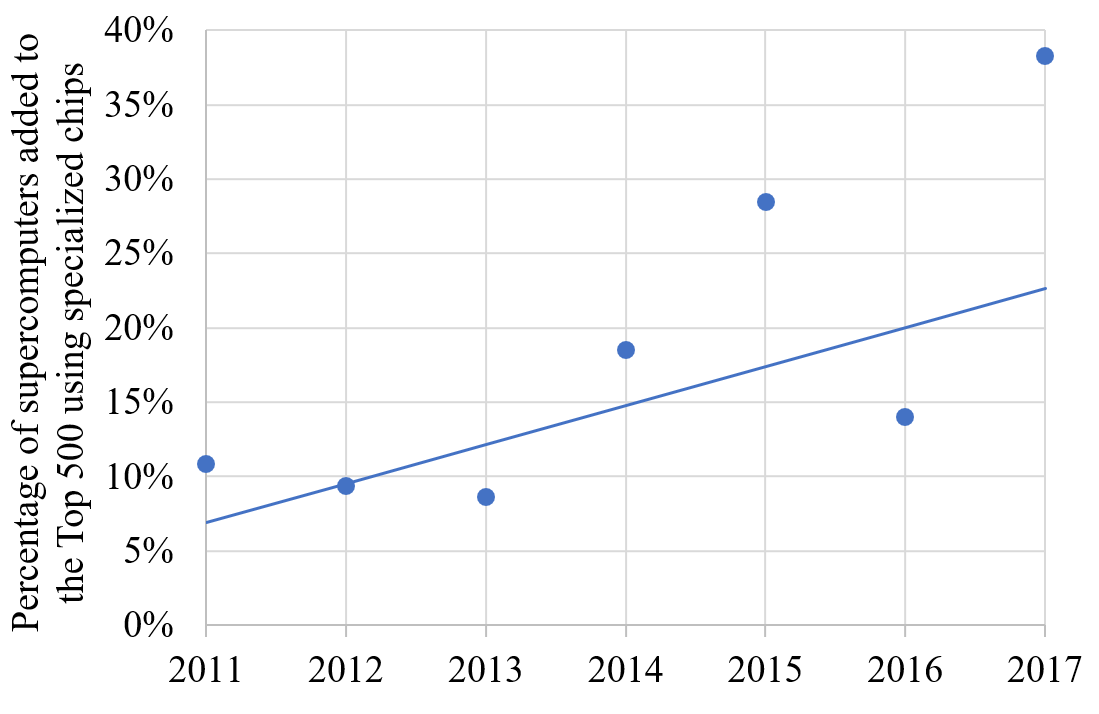
\includegraphics[scale=0.4]{figures/Supercomputers-with-pecialized-chips.png}
    \caption{Graph showing increasing popularity of 
specialized hardware in high performance computing \citep{GenPurpTech}.}
    \label{fig:1}
\end{figure}

\section{FPGA Overview}
A field-programmable gate array, or FPGA, is a digital integrated circuit that consists of millions of logic blocks that can be configured to perform different operations. The process of configuring the logic blocks is called FPGA design and can be compared to the design of integrated circuits. Reconfigurability and ease of design are the main advantages when using an FPGA as a computing platform. When comparing an FPGA design with a solution that is developed using software, the FPGA stands out with process pipelining and a high level of parallel processing. The difference between executing a software program on a processor and executing the equivalent operation on an FPGA is that the compiled software instructs the processor to do operations in a generic way, as in loading a register and shifting a bit. An FPGA does not need to explicitly load a register, because the registers are by default connected to the input of the operation, which is defined by the FPGA design. A bit shift operation is typically an inexpensive operation regardless of the computing platform, but the FPGA can pipeline the result directly into another register or operation, which saves clock cycles. The pipeline principle is demonstrated in Figure \ref{fig:pipeline} by comparing it with a non-pipelined solution. The pipeline transformation enables the inactive parts of the calculation to be utilized when they would normally be idle, waiting for all parts to finish. \citep{XilFPGAIntro}

\begin{figure}
    \centering
    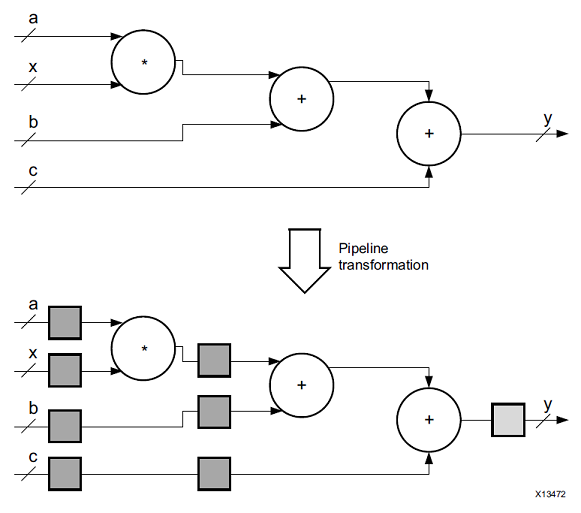
\includegraphics[scale=0.7]{figures/structure_fpga_imp_compute_function.png}
    \caption{Figure showing two execution paths for the expression $y=(a \times x) +  b + c$. The operations on the first path depend on the output from previous operations, whereas the operations on the second path depend on separate input register. The second path is a pipeline transformation of the first path. \citep{XilFPGAIntro}}
    \label{fig:pipeline}
\end{figure}

% Volatile vs non volatile FPGA (SRAM, flash, anti-fuse)
% https://www.edn.com/a-comparison-of-space-grade-fpgas-part-1/
% https://www.edn.com/fpga-architectures-from-a-to-z-part-1/
% https://www.eetimes.com/all-about-fpgas/#
% FPGA Interconnect
% IO Cell, clocks http://xilinx.eetrend.com/files-eetrend-xilinx/forum/201509/9204-20390-7_series_architecture_overview.pdf
% https://nanopdf.com/download/fpga-programmable-interconnect-and-i-o-cells_pdf
% https://www.analog.com/en/analog-dialogue/articles/care-and-feeding-of-fpga-power-supplies-a-how-and-why-guide-to-success.html

\par
Xilinx is one of the key companies involved in FPGA production, both currently and historically. They introduced the world to FPGAs in 1985 and have since then led the programmable logic technology industry, with a 51\% market share of programmable logic device suppliers in 2017. Major end market categories for Xilinx are aerospace, defense, and communications. The main competitor of Xilinx is Intel with a market share of 37\%. \citep{XilHist}\citep{XilShare}
\par 
Due to the significance of Xilinx, and relevancy in this project, FPGA technology discussed in this work is Xilinx based. Differences between manufacturers include technological and architectural nuances. For example, Xilinx exclusively manufactures static random-access memory (SRAM)-based FGPAs. This refers to the technology of the programmable parts of the FPGA. Other available technologies are flash and anti-fuse, which are less common than SRAM. \citep{FPGAarch1}
\par
The basic internal elements of an FPGA consist of circuits such as look-up tables, flip-flops, wires, and input/output pads. Using these elements the FPGA design is implemented in the hardware.
The architecture is illustrated in Figure \ref{fig:2} which shows a matrix arrangement of configurable logic blocks which are connected to each other with an interconnect, consisting of wires and switch matrices. The wires also run to the input/output pads, which enables interfacing with off-chip components such as synchronous dynamic random-access memory (SDRAM) or sensors. Configurable logic blocks (CLBs) contain the look-up tables and flip flops. An overview of a CLB is shown in Figure \ref{fig:3}. \citep{XilFPGAIntro}

\begin{figure}[h]
    \centering
    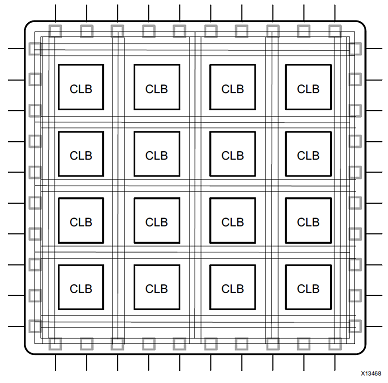
\includegraphics[scale=0.55]{figures/basic_fpga.png}
    \caption{FPGA architecture. An FPGA consists of configurable logic blocks, input/output pads, and an interconnect \citep{XilFPGAIntro}.}
    \label{fig:2}
\end{figure}

\begin{figure}[h]
    \centering
    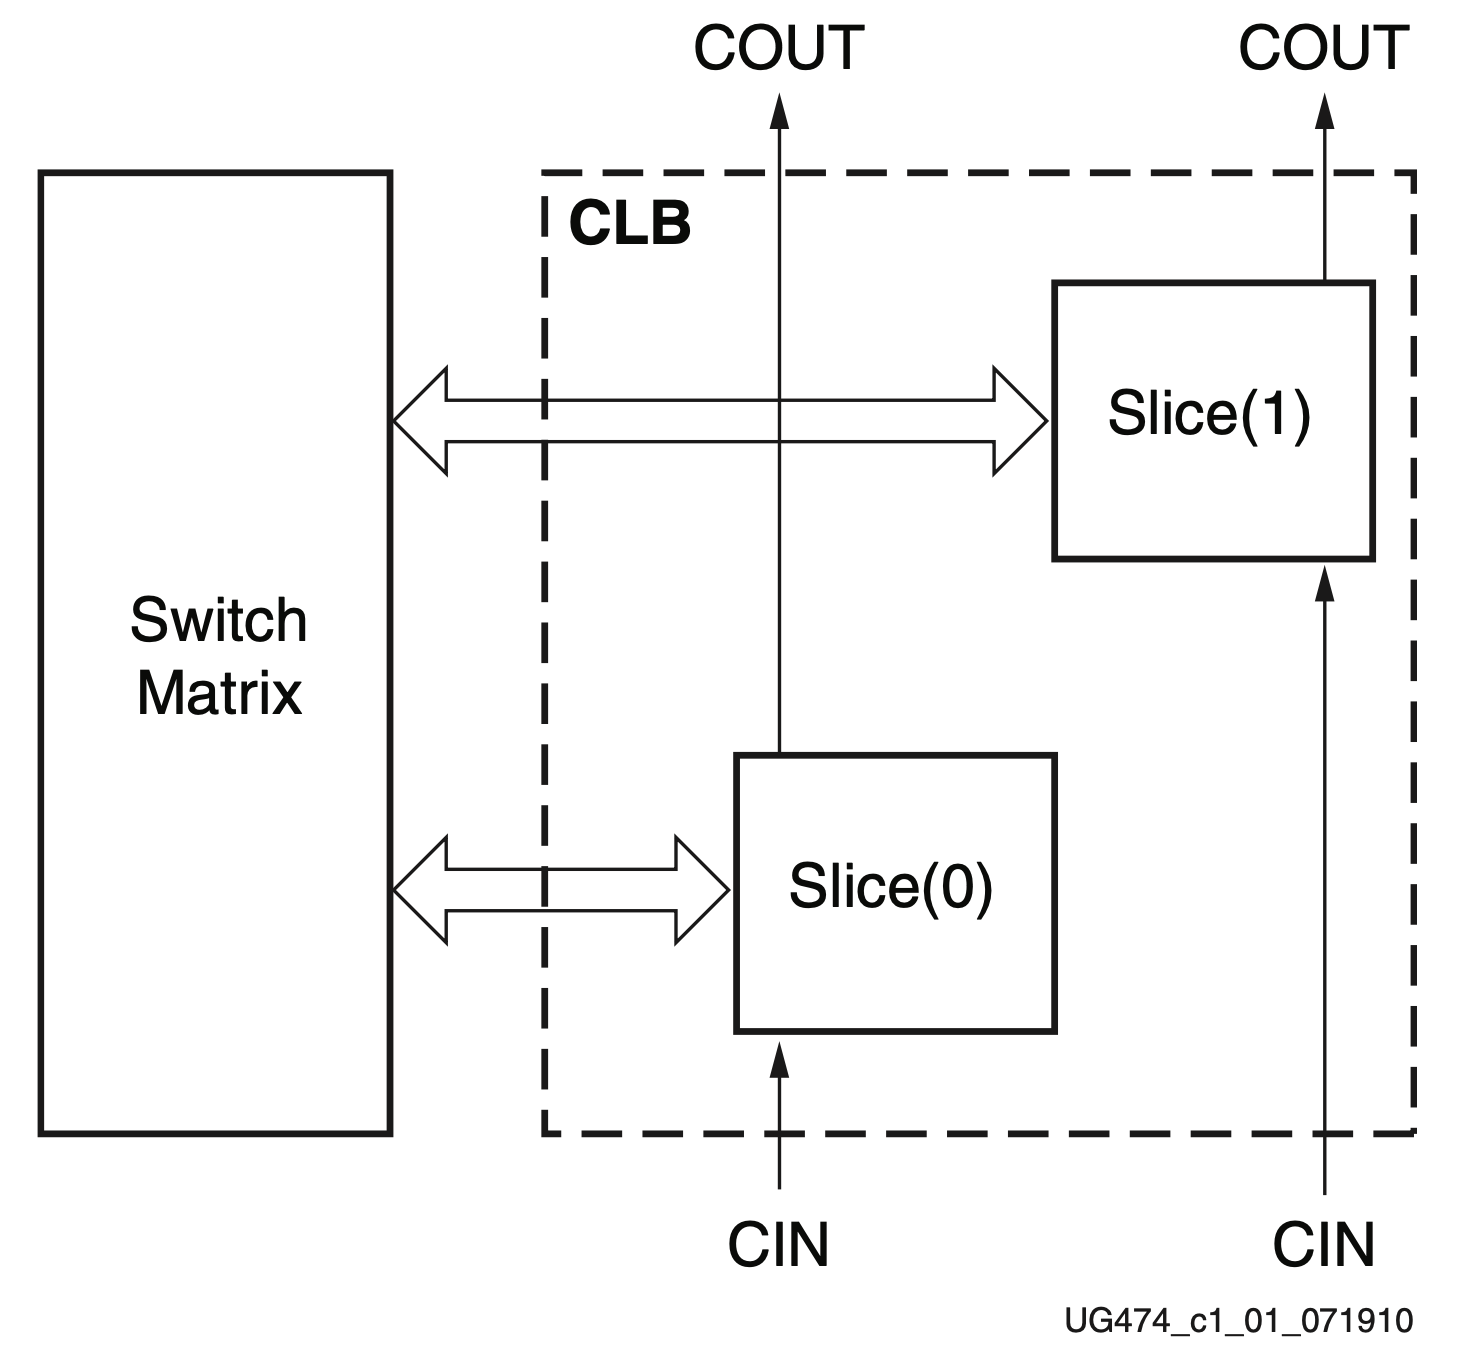
\includegraphics[scale=0.25]{figures/clb.png}
    \caption{Diagram of a configurable logic block. A CLB consists of logic element containers, called slices, inputs, and outputs. Both slices are attached to the switch matrix, connecting the CLB to other CLBs. \citep{XilClbMan}}
    \label{fig:3}
\end{figure}

The slices in Figure \ref{fig:3} represent core elements of an FPGA. Slices consist of look-up tables, storage elements, multiplexers, and carry logic. Depending on the FPGA, there are different numbers of slices per CLB. The slices are collectively responsible for implementing a significant portion of the FPGA design. \citep{XilClbMan}
\par
Look-up tables (LUT) are mainly used as logic elements in FPGAs. They can implement any boolean logic operation by combining memory cells with multiplexers. A look-up table is essentially a truth table that can be used for reading the result of boolean operations. Memory cells and multiplexer routings are initialized by the FPGA design, which is what makes the look-up table element configurable. An example of a four memory cell wide LUT is shown in Figure \ref{fig:4}. \citep{XilFPGAIntro}

\begin{figure}[h]
    \centering
    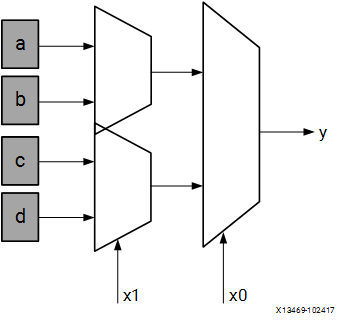
\includegraphics[scale=0.5]{figures/lut.png}
    \caption{Example of a look-up table with four memory cells and two multiplexers. The FPGA design initializes memory cells \textbf{a-d} and uses inputs \textbf{x1} and \textbf{x0} to select value \textbf{y}. \citep{XilFPGAIntro}}
    \label{fig:4}
\end{figure}

The circuit elements discussed in this chapter form the basic blocks of FPGA technology. A larger set of elements are often included in an FPGA to enable some optimizations and further functionality in the design. For example, there are different types of slices a CLB can contain, which make it more suitable for storage purposes rather than logic. Signal processing pipelines are a popular use case for FPGAs and they often contain slices specialized for operations in this problem domain. Digital signal processing can be accelerated by parallelizing operations in a single instruction multiple data (SIMD) fashion, thus to maximize signal processing performance a large number of this type of slices is found in FPGAs. Figure \ref{fig:5} shows an example of an FPGA configuration with some of these specialized blocks mapped out. The green CLBs are designated to memory usage and are closely coupled to the red digital signal processor (DSP) blocks to enable fast processing of the stored data. The purple external memory controllers use the input/output pads to interface with external memory such as SDRAM. \citep{XilFPGAIntro} \citep{XilClbMan}

\begin{figure}[h]
    \centering
    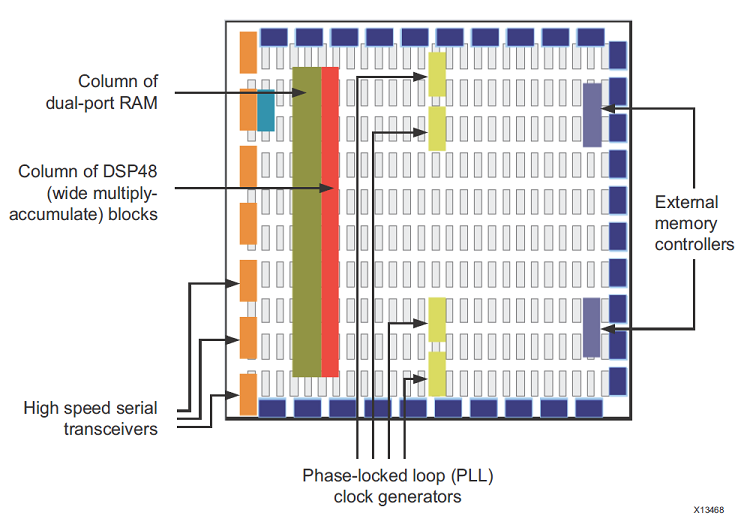
\includegraphics[scale=0.5]{figures/contemporary_fpga.png}
    \caption{DSP system design on FPGA \citep{XilFPGAIntro}.}
    \label{fig:5}
\end{figure}

When comparing FPGAs with each other the main performance metrics are power consumption and number of logic cells. The number of logic cells determines the size and complexity of the design that the FPGA can fit. Additionally, the FPGAs can often be compared by specifications such as specialized CLB slices, I/O interfaces, and communication rates. Clock speed is seldom compared because although there is an upper limit, it is often design specific. \citep{XilClbMan} \citep{XilFPGAIntro} 

\section{System design with HDL}
The main tool for creating an FPGA design is a hardware description language (HDL). VHDL and Verilog are examples of commonly used HDLs. Compared with conventional computer programming languages, HDLs are used in a data flow fashion to describe the timing and logic of an integrated circuit. The data flow description of a circuit in an HDL is such that all code blocks are executed simultaneously by default. This is one of the main advantages of FPGAs as the system is inherently parallelized. It creates also one of the biggest challenges in HDL based design as it complicates the timing of events and resource concurrency.
\par
The output of an HDL design is produced by a build process that computes the high level data flow description into low level circuit elements and routing. This can be compared to the compilation phase of code written in a statically typed software programming language. 
\par
The synthesis process is where the HDL design known as register transfer level code is transformed to a gate level description called netlist. The netlist is a mapping of circuit components that are found inside the FPGA. The convenience of HDL based design is being able to describe the circuit at a higher level. In practice this means that registers and buses are created and connected to be inferred into low level circuitry at the synthesis phase. When developing a design against a specific FPGA, a bitstream file is created to configure the device with. The end product of an HDL based design is the bitstream file or, alternatively, the synthesis result as it can be used for simulation purposes by a test bench. \citep{XilVivado}

\section{System design with IP cores}
Designing a hardware system often involves components of a reusable nature, such as dividers, communication protocols, and memory controllers. Intellectual property (IP) cores are distributions of components such as these. An IP core can be of varying complexity as it can consist of a solution for a specific task or describe a complete system on a chip (SoC). IP cores are licensed through a patented design which is what the name refers to. They can often be configured to suit different properties of the implementation such as data width and clock rate. The core is then connected to the system using an HDL. The core itself may consist of software or hardware macros. The software macro, or soft IP core, is an HDL implementation of the IP core logic that is built to the specific FPGA with the rest of the system design. A hardware macro, or hard IP core is prebuilt and FPGA specific. \citep{EERefBook} \citep{XilVivado}
\par
The hardware sector and consumer electronics industry rely heavily on reusable IP cores. For example, the SoC or motherboard found in mobile phones often includes advanced RISC machine (ARM) based processor cores licensed from ARM holdings. The producer of the mobile phone benefits from avoiding the development of the processing unit but still has the ability to customize the SoC to a high degree by combining different processing units, memories, and other IP cores. Figure \ref{fig:6} shows the architecture of an SoC which has an ARM based CPU, and other modules commonly found in mobile phones. In addition to the CPU, any of the remaining modules might also be licensed IP cores. \citep{ArmInMobile} \citep{HarvIPCore}

\begin{figure}[h]
    \centering
    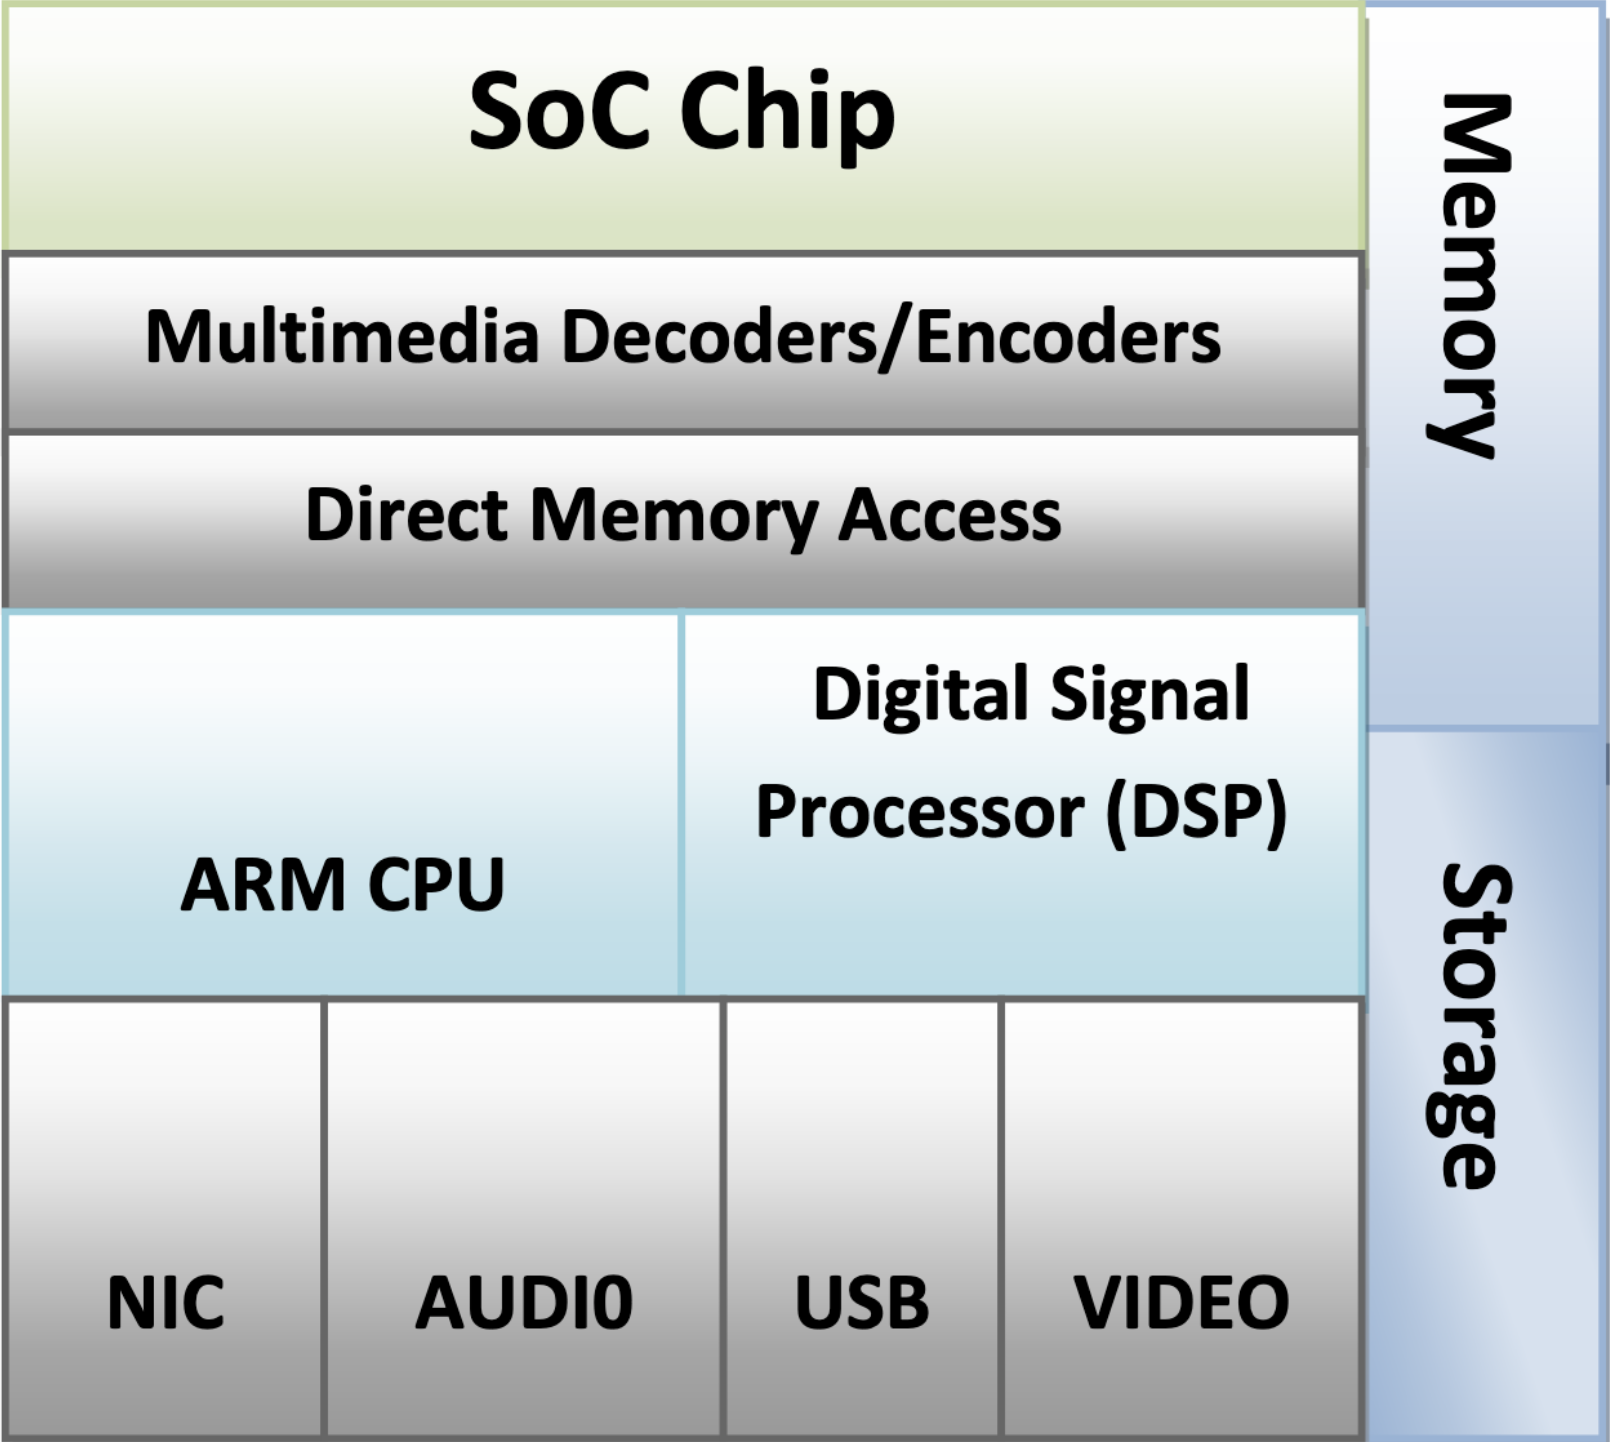
\includegraphics[scale=0.25]{figures/arm_soc.png}
    \caption{Common SoC found in smartphones includes ARM based CPU and DSP. \citep{ArmInMobile}}
    \label{fig:6}
\end{figure}

\par
In aerospace applications, the advantages of IP cores are utilized in the same manner as within the mobile phone industry. Additional requirements such as fault tolerance limits, redundancy, and formal verification of the IP cores increase the advantages of their usage when comparing with in-house developed solutions. This, however, comes with pricier licenses compared with non-aerospace grade IP core designs. Also, due to the specialized requirements, lower competition in the market sector can be expected, increasing the prices even more. \citep{DO254Cadence}
\par
In addition to FPGA products, Xilinx also provides design tools and IP cores to help with development on their FPGA platforms. A selection ranging from small subsystem designs to complex embedded processors is available through the Xilinx IP core library. Some of the cores are available free to use through the Vivado design suite, and a majority of them are soft cores to allow compatibility across their FPGAs. Integration of the IP cores and other development are also done through Vivado. \citep{XilVivado}
%OPENCORES
% https://www.xilinx.com/content/dam/xilinx/support/documentation/white_papers/wp523-xqrku060.pdf
% https://www.techspot.com/article/1989-arm-inside/
% https://www.techspot.com/article/1821-how-cpus-are-designed-and-built/
%The image processing pipeline uses three different storage mechanisms. 
%\subsection{SDRAM}
%The main working memory of the image processing pipeline is a off-chip 512MiByte, 32-bit wide DDR3 SDRAM memory module.
%\subsection{BRAM}
%\subsection{FIFO}
%\subsection{PipeIn/PipeOut}

%\section{Licensing and standards}
%\subsection{IEEE}
%\subsection{ISO}
%\subsection{DO-254}
% https://www.cadence.com/content/dam/cadence-www/global/en_US/documents/solutions/aerospace-and-defense/do-254-explained-wp.pdf
% https://people.duke.edu/~goodw010/Wiki/hwswstds.html
%\subsection{MIL}

\chapter{System requirements}

A hardware implementation of an image analysis software component is to be developed to be used on an FPGA. The software in question is a product of a research project regarding detection and analysis of space debris in low earth orbit. Using computer vision among other analysis, space debris is identified from image data. With the help of a star catalog, the image is mapped to a position in space to provide positional data of the detected debris. A diagram of the system is shown in Figure \ref{fig:0}. The software component relevant to this project is the pre-processing and segmentation part of the diagram, which is in the input phase of the complete system. \citep{StreakDet} \citep{Starmatch}

\begin{figure}[h]
    \centering
    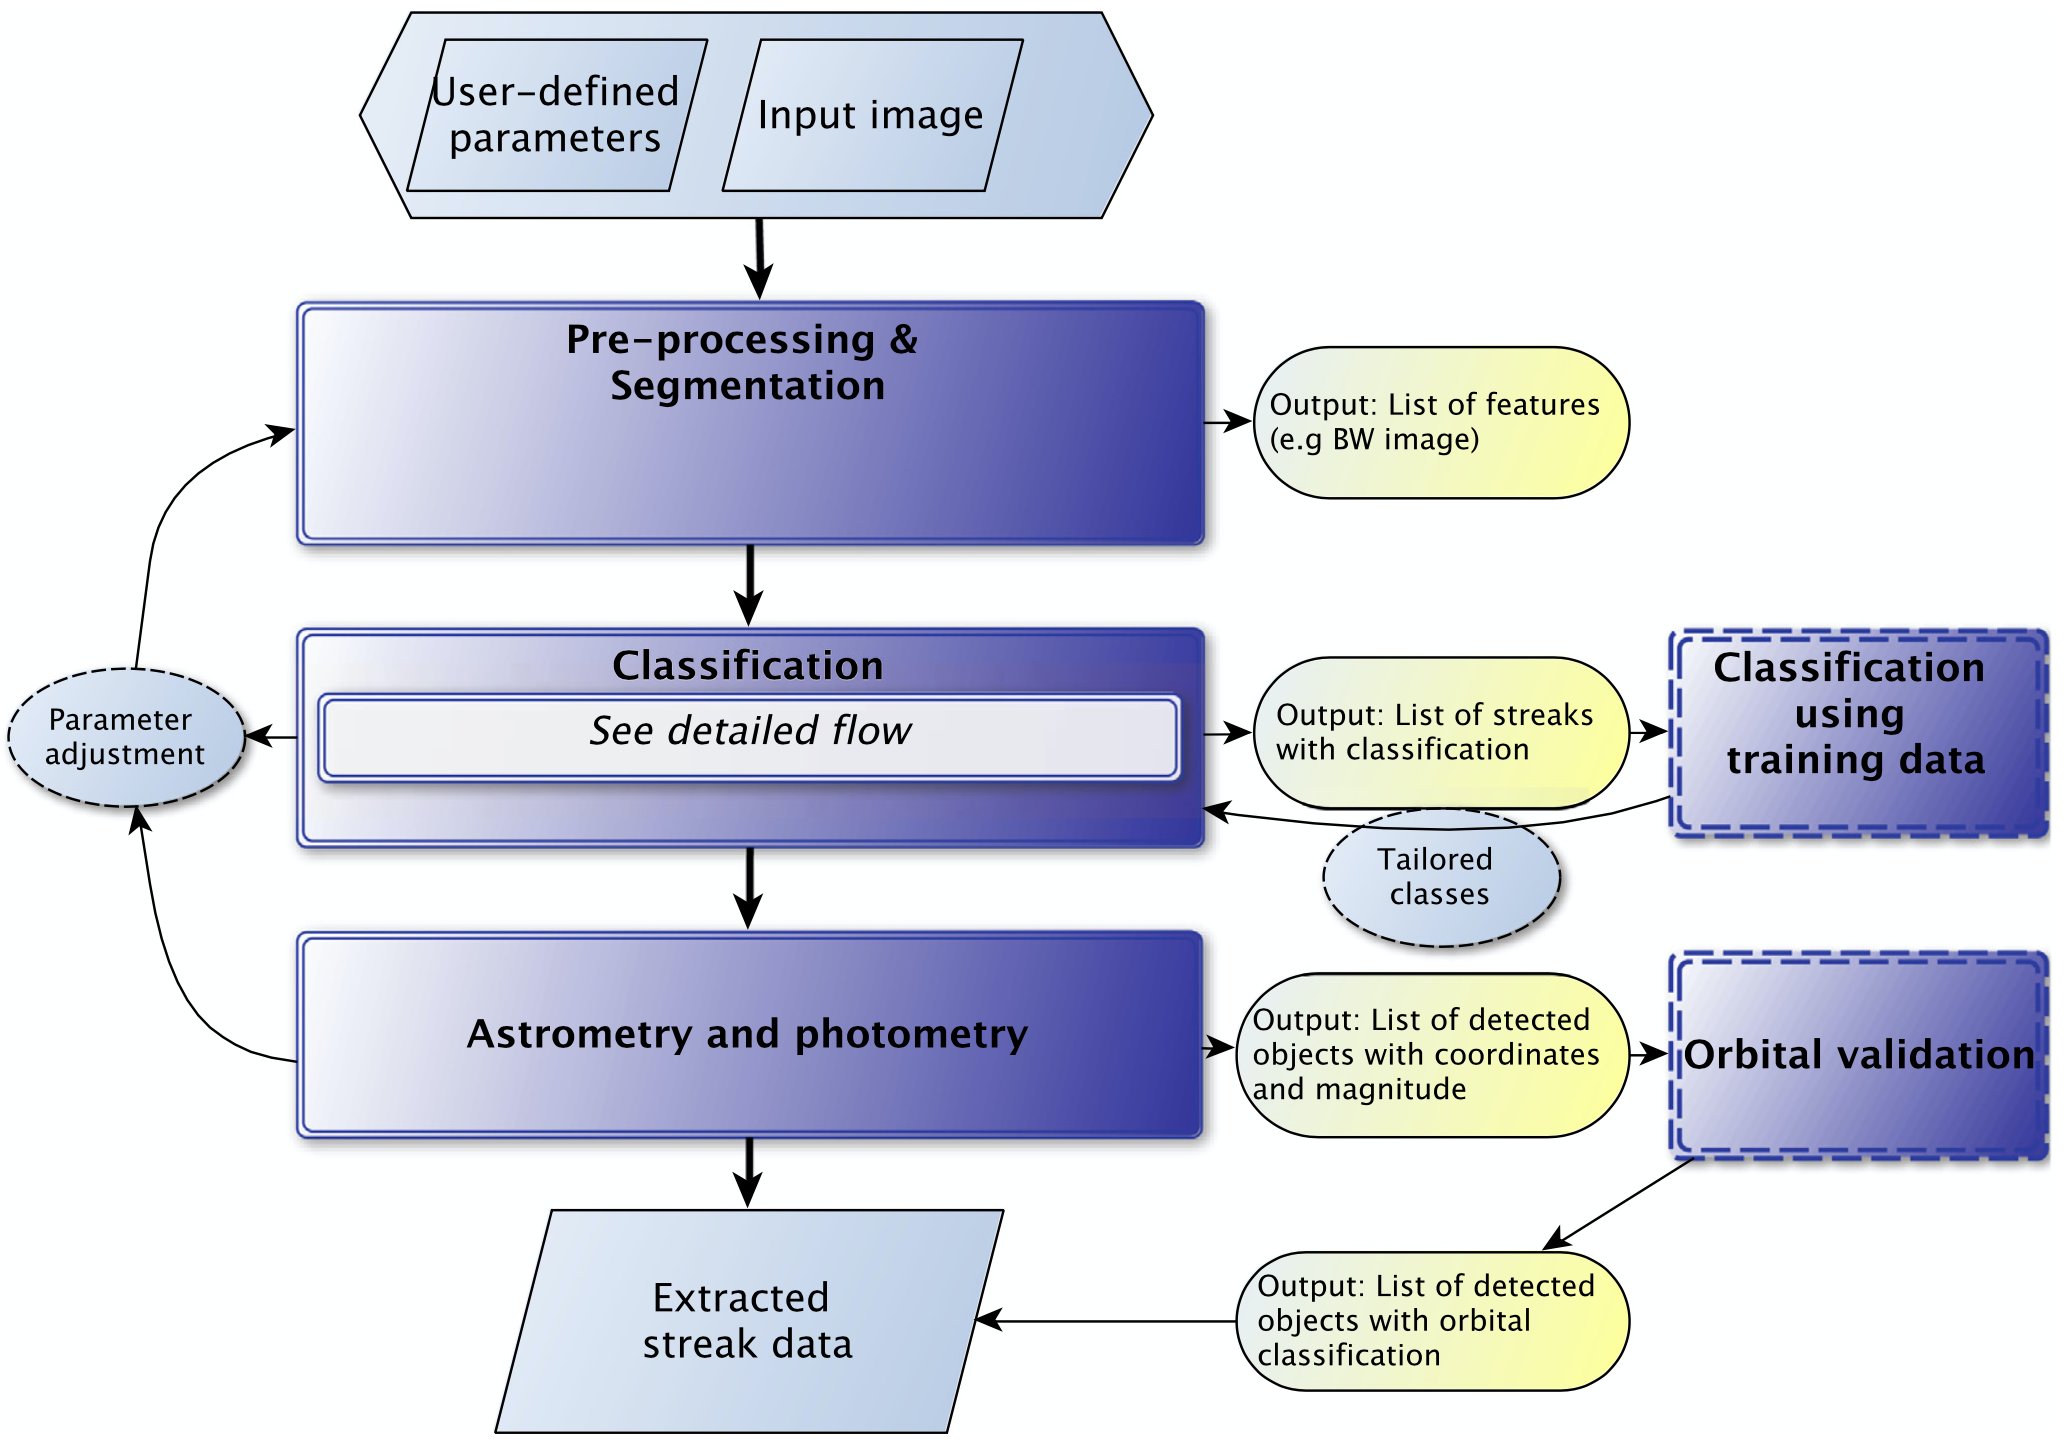
\includegraphics[scale=0.2]{figures/streakdet.png}
    \caption{Flowchart of StreakDet software \citep{StreakDet}.}
    \label{fig:0}
\end{figure}

%\section{Scope}
The star extraction process in StreakDet passes the input image through a series of algorithms to identify stars. The algorithms are well-known image filters and analysis methods that in combination with each other produce a way to extract objects from an image. The main task in this project is to implement the algorithms to a hardware design using a hardware description language.
\par
Star extraction is a key stage of a star tracker system which uses a star catalog to match the extracted stars against. Using the star matches and catalog information the position and orientation of the captured image can be determined. The goal of this project is to create a pre-processing pipeline to be used in a star tracker.

\section{System specification}

The specification consists of development and system requirements as well as a description of tools and components. System requirements are created based on meetings and discussions with Aboa Space Research Oy. Some requirements are derived from higher level requirements to suit the development process. Table \ref{table:sysreq} presents an overview of the system.

\begin{table}[h]
    \begin{tabular}{|p{1.75cm}|p{10cm}|}
        \hline
        \textbf{Req. Id}& \textbf{Description}\\
        \hline
        \hline
        \textbf{1}&Client endpoint for FPGA module\\
        \hline
        1.1\label{req1.1}&Bitstream can be written to FPGA\\
        1.2\label{req1.2}&Image processing pipeline parameters can be written to FPGA\\
        1.3\label{req1.3}&Allows for debugging of system\\
        1.4\label{req1.4}&Provides visual results with metadata\\
        \hline
        \hline
        \textbf{2}&Validation and verification of star extraction\\
        \hline
        2.1\label{req2.1}&First stage validation and verification with software prototype\\
        2.2\label{req2.2}&Second stage validation and verification on FPGA platform\\ 
        \hline
        \hline
        \textbf{3}&Star extraction result and operation\\
        \hline
        3.1\label{req3.1}&Image coordinates of extracted stars are stored\\
        3.2\label{req3.2}&Centroid of detected stars is calculated\\
        3.3\label{req3.3}&Error handling to avoid false detection\\
        \hline
    \end{tabular}
    \caption{System requirements specification}
    \label{table:sysreq}
\end{table}

%The development requirements involves critical steps that are necessary when working towards the system requirements.
%\subsection{Scope}
%\subsection{Image processing pipeline stages}
\subsection{System components}
\subsubsection{Processing nodes}
The system consists of two nodes, the host machine and the target FPGA. Because the application of this system will be different in a production environment, the FPGA part should not be too dependent on the host machine. When integrated into a larger system with shared memories and communication, the FPGA will have to be able to read an input image directly from memory. The same applies to the output, the register where the output is written needs to be configurable and not sent to a host machine by default.

\subsubsection{FPGA module}
The FPGA module Opal Kelly XEM7305 chip with a Xilinx Spartan-7 FPGA will function as a testbed for development. The module contains a part from the FPGA external SDRAM memory and communication interfaces such as USB 3. These features allow for host machine communication and data storage of features such as images, star catalog, and output. These data could be stored on the FPGA itself but using the SDRAM is a sustainable solution because it allows for shared memory usage in production and more flexible image and star catalog sizes.


\chapter{\mbox{FPGA-based computer hardware}}
Common computer hardware is the cornerstone of any digital circuit that needs to perform common tasks, such as storing and transmitting data. With the help of the basic elements of an FPGA discussed in Chapter 2, circuits of this nature can be created. Although an 8-bit adder circuit can be regarded as common computer hardware, the focus of this chapter is on larger circuits used as hardware modules, such as memory and communication interfaces. The components discussed are essential building blocks for the image processing pipeline. Figure \ref{fig:xemOverview} shows an overview of these components on the XEM7305 FPGA module.

\section{Communication}
The system requirements state a communication channel to be available for shared memory usage and controlling the FPGA. Machine-to-machine communication is enabled through the interfaces available on the Opal Kelly FPGA module. The default interface on XEM7305 is USB C. \citep{XEM7305Man}
\par
The advantage of the USB is flexibility and ease of use. Transfer speed is not a high priority in this case because of the relatively small size of data, which is less than a megabyte. The USB module on the XEM7305 contains a USB C port and a Cypress FX3 peripheral controller, shown in Figure \ref{fig:xemOverview}.
The peripheral controller operates the data bus by implementing a communication protocol stack consisting of a physical, link and protocol layer. It allows the usage of the USB communication link on the FPGA module by exposing a programmable interface. The programmable interface can be used by various systems on the FPGA module, such as an image sensor or the FPGA itself. To allow the usage of the programmable interface of the peripheral controller in the FPGA design, a hard IP core is provided. \citep{XEM7305Man} \citep{FX3Man}

\begin{figure}
    \centering
    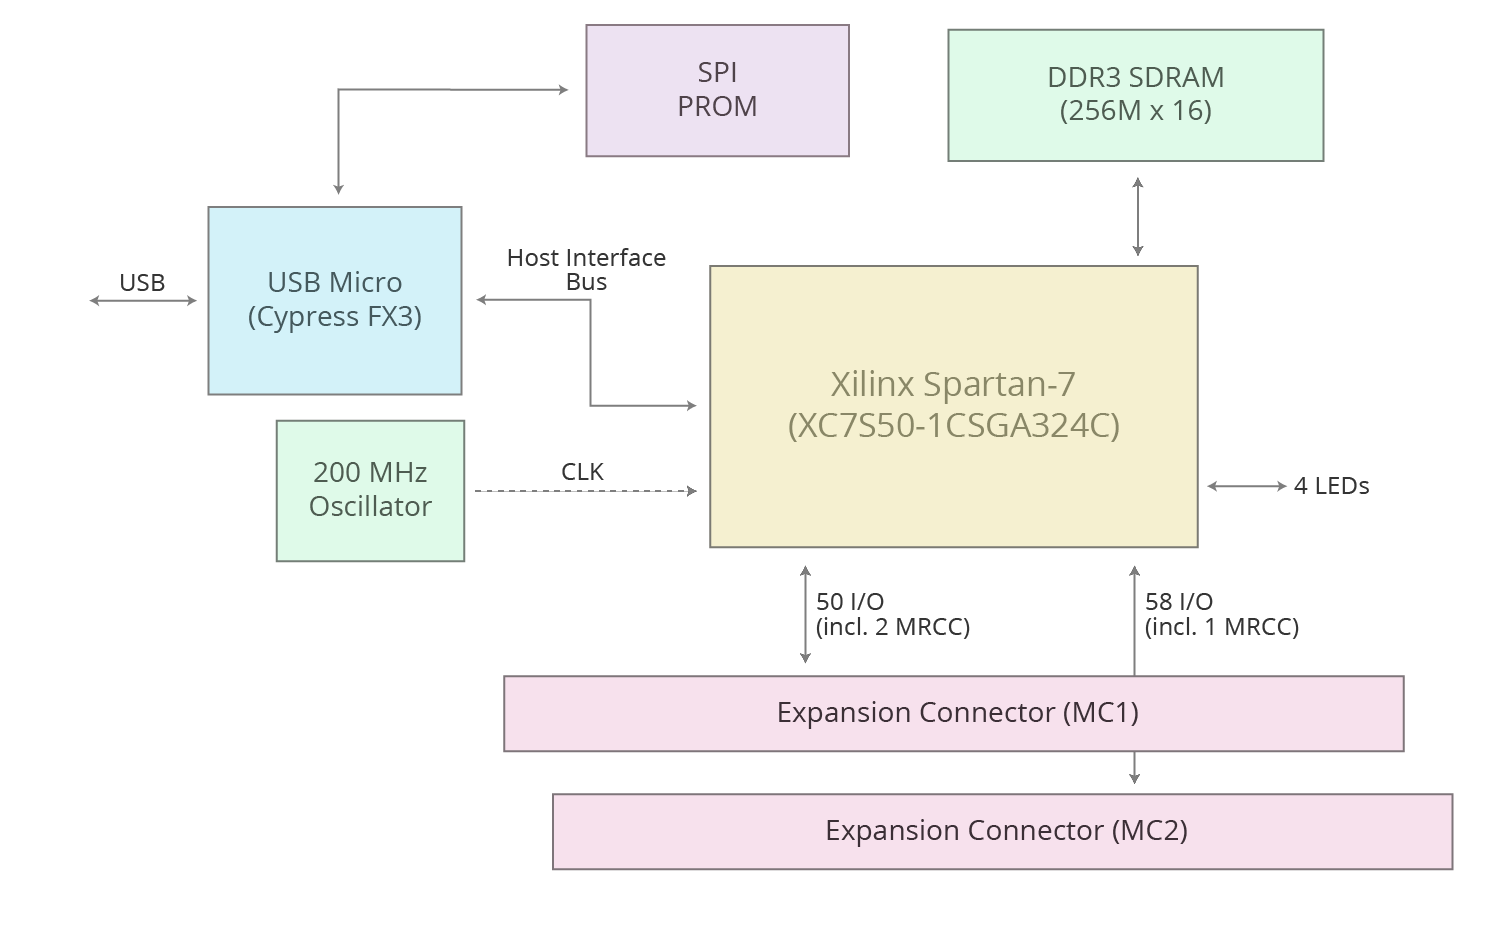
\includegraphics[scale=0.4]{figures/2XEM7305-BlockDiagram.png}
    \caption{Overview of the FPGA module showing the FPGA itself in the center, SDRAM off-chip memory on the top right, and USB interface on the left. \citep{XEM7305Man}}
    \label{fig:xemOverview}
\end{figure}

Both the USB 3 standard and the FX3 peripheral controller support serial and parallel communication, but the hard IP core connecting to the FX3 interface supports only serial communication. This simplifies the use of the IP core, requiring less FPGA fabric, but also reduces the throughput. \citep{XEM7305Man} \citep{FX3Man}

\par
The internal communication mechanism of an FPGA consists of the FPGA interconnect. The interconnect is the physical layer of the communication protocol stack, leaving the rest of the stack to be implemented in the FPGA design with HDL or IP cores. 
\par
The limiting factor and bottleneck of the system is often some off-chip hardware module that places certain requirements on the communication, for example, the USB or memory controller. When working outside these types of requirements, the throughput of the FPGA-based system can be optimized by increasing the bit width between modules. When applying this to the image processing pipeline context, this might be practical within communication of image data. The implementation of this requires more memory cells and wires which, in turn, increases the footprint of the FPGA design.
\par
When compared with a software program, the same optimization method of maximizing bit width might be considered. This, however, does not inherently result in a gain in throughput because conventional CPUs have a fixed bit width for their operations. When this limit is exceeded, the operation needs to be performed across multiple clock cycles which counteracts the wanted result. The bit width of an operation on an FPGA during a clock cycle, is consistent with the HDL design. 
\par
% Image of low vs high bit width circuit/ footprint
% More in depth on USB3, images
% https://www.usb.org/sites/default/files/CabConn_3_0_Compliance_Document_20101020.pdf
% https://www.usb.org/documents?search=&category%5B%5D=49&tid_2%5B%5D=39&items_per_page=50
% PipeIn PipeOut
% Cypress FX3 Microcontroller

\section{Memory}
To enable processing of image data, a set of storage mechanisms is necessary. The use of a certain memory type is mostly dependent on the size of the data and how it will be used. As in conventional CPU architectures, different levels of memory are used to satisfy these dependencies.
\par
FPGAs are generally not well suited for storing a large quantity of data, as it is considered inefficient use of available CLBs. Since customization is a key feature, the most standardized parts, such as memory, are often placed outside the FPGA. Off-chip memory allows storage of large data, such as images, freeing up CLBs to other usage such as computation and logic. The drawback with off-chip components is that they are often a bottleneck in the system. This is due to a number of factors such as restrictions in clock speed, concurrency, and bus width. A larger FPGA with an increased number of CLBs could offset the need for off-chip memory avoiding the bottleneck, with consequences being greater power consumption and physical size, potentially invalidating the solution.
\par
An overview of the XEM7305 module and the memory types can be seen in Figure \ref{fig:xemOverview} where the off-chip SDRAM memory is on the top right and the lower level memories inside the Xilinx Spartan 7 FPGA in the center.

\subsection{SDRAM}
One of the most common storage mechanisms is SDRAM which is useful for storing data that is frequently used and ranges from kilobytes to megabytes in size. Key features include random access, i.e. same access time for any part of the memory, and high bandwidth. It is often paired with FPGAs, because it is next in the memory hierarchy after on-chip storage mechanisms.
\par
At the core of SDRAM lie capacitors trapping the charge representing a bit. An overview of a typical SDRAM circuit is shown in Figure \ref{fig:7}. The capacitors are refreshed periodically to retain the stored data. This makes SDRAM a volatile memory, requiring power to keep its state. The advantage over closely related memory types, such as flash memory, is that it does not degrade at the same rate of read/write cycles and it is truly random access, giving the advantage to SDRAM as a volatile working memory in most FPGA applications. \citep{SDRAMFLASH} \citep{NANDNORFlash}

\begin{figure}[h]
    \centering
    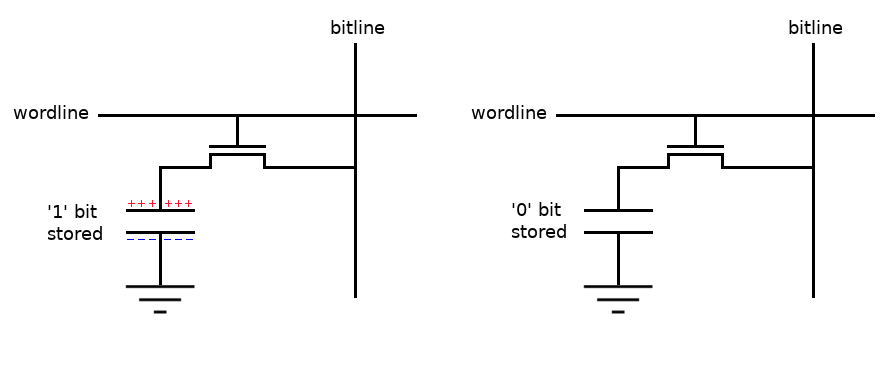
\includegraphics[scale=0.4]{figures/DRAM.jpg}
    \caption{SDRAM memory cell. The capacitor traps the charge which is controlled by the transistor at the top. \citep{SDRAMFLASH}}
    \label{fig:7}
\end{figure}

The memory cells in SDRAM are ordered in rows and columns, forming an array. A collection of these arrays is referred to as memory banks. 
%\begin{wrapfigure}{r}{0.5\textwidth}
%\end{wrapfigure}
The number of rows, columns, arrays, and banks varies depending on the type of SDRAM but is usually a power of two. Figure \ref{fig:8} shows the geometry of an SDRAM with four banks with four arrays each. The data width of a memory is the number of arrays that are stacked inside each memory bank. When accessing a specific row and column, the number of affected bits is the same as the data width of the memory.
\par
To increase SDRAM performance, double data rate (DDR) is used to access data at double the clock rate. DDR enables accessing a memory bank on both the rising and falling edge of the clock cycle. A prefetch mechanism enables the transfer of multiple bits concurrently per bank access, increasing the throughput even more. This mechanism enables efficient use of the internal SDRAM bus width by also transferring data from neighboring addresses. The gain comes from the fact that the time to access a single address is the same as accessing the neighboring ones as well. The prefetch mechanism gives an advantage to data which is structured in a way where each access is in adjacent addresses. The width of the prefetch data depends on the DDR version. Other variations between DDR versions are the supported clock frequency and burst length, which are features related to the prefetch mechanism. The burst length specifies the number of SDRAM words contained in each read or write operation. \citep{MicronSDRAMGeneral}

\begin{figure}[h]
    \centering
    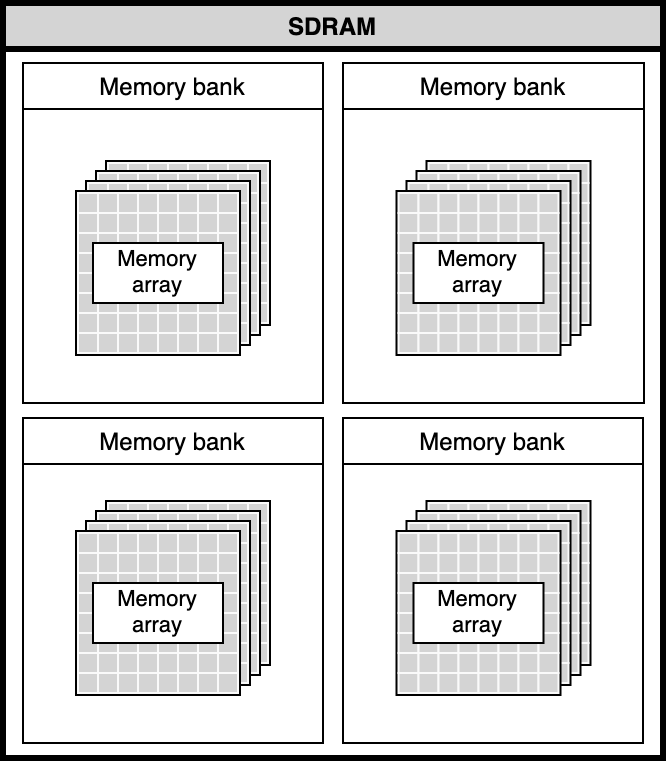
\includegraphics[scale=0.3]{figures/sdram_bank_array.png}
    \caption{SDRAM geometry.}
    \label{fig:8}
\end{figure}

The XEM7305 features a Micron DDR3 SDRAM chip with a 32-bit wide interface. The memory part has 8 banks, 32 768 row addresses, 1024 column addresses, and 16 bits to each address, giving the a capacity of 4Gb. As previously discussed, the DDR version dictates the prefetch data width, which in DDR3 is 8 words, as is the burst length. The word length of the memory is 16 bit, which results in 128-bit burst transfers. The SDRAM is rated with a clock frequency of 1600 MHz, giving a theoretical peak bandwidth of 3.2 GB/s. In practice, the bandwidth is lower and depending on system state and access location. \citep{XEM7305Man}
\par
The oscillator on the FPGA board provides a 200 MHz signal, which is also the limit of the Spartan 7 FPGA. This allows a maximum clock frequency of 325 MHz to be generated through the SDRAM controller interface and then scaled up to 650 MHz with DDR at the SDRAM.
\citep{XEM7305Man} \citep{MicronSDRAM}
\par
The memory controller interface connects the FPGA to the SDRAM controller, which in turn sends commands to the SDRAM core. The interface is unique to each memory controller and depends on all parameters discussed in this chapter such as memory geometry, DDR version, and clock frequency. \citep{XEM7305Man}

%((32k * 1k)*8) = addr
%addr * 16 = capacity

%https://www.xilinx.com/support/documentation/user_guides/ug473_7Series_Memory_Resources.pdf
%https://user.eng.umd.edu/~blj/memory/Book-Overview.pdf
%https://www.allaboutcircuits.com/technical-articles/executing-commands-memory-dram-commands/
%http://taututorial.yolasite.com/sdram-controller.php
%https://itectec.com/superuser/how-to-interpret-the-parameters-in-a-dimm-datasheet/
%https://www.micron.com/-/media/client/global/documents/products/technical-note/dram/tn4605.pdf
%https://www.es.ele.tue.nl/premadona/files/akesson01.pdf
%https://www.design-reuse.com/articles/13805/the-love-hate-relationship-with-ddr-sdram-controllers.html

\subsection{Block RAM}
When data size is within a few megabytes or less, lower level storage mechanisms become suitable to use as memory. The block random-access memory (BRAM) is a type of on-chip memory, which uses memory cells available on the FPGA. The specification of an FPGA chip often includes the available BRAM capacity. Although BRAM is a type of on-chip memory, it is separate from the CLBs on the FPGA. In the case of SRAM based FPGAs, the memory cells of the BRAM are essentially SRAM cells, arranged in arrays. The BRAM is made available to the other CLBs by being attached to the FPGA interconnect.
\par
BRAM can be configured in size and functionality depending on the needs. Common BRAM arrays are 36Kb that can either be divided into smaller arrays, or combined with other arrays to form a larger memory resource. A useful feature often found regarding BRAM is multiport support. This enables concurrent usage of the memory resource. In case of concurrency issues, the configurable operation mode of the BRAM dictates how to resolve them. For example, in a dual port configuration, the read first operation mode will prioritize a read operation when the other port requests a write operation on the same address. \citep{XilMemMan}
\par
% example configuration & geometry
\par
Similarly as SDRAM, BRAM also is synchronous and requires a clock signal. The latency depends on the configuration and state of the memory, but is usually within a few clock cycles. The low latency, together with the high configurability, makes BRAM a useful resource in most FPGA designs. \citep{XilMemMan}

% shift register vs block ram
% https://www.xilinx.com/support/documentation/white_papers/wp377_7Series_Embed_Mem_Advantages.pdf
% https://eprint.iacr.org/2018/717.pdf
% https://archive.org/details/eu_SciAm_1997-06_OCR/page/n55/mode/2up?q=configurable+computing+scientific+america
% http://www.righto.com/2020/09/reverse-engineering-first-fpga-chip.html
% https://ieeexplore.ieee.org/document/6487750?reload=true
% https://www.xilinx.com/support/documentation/ip_documentation/blk_mem_gen/v8_3/pg058-blk-mem-gen.pdf
\subsection{Distributed RAM}
The lowest level of memory found in FPGAs is distributed RAM (DRAM). It is a type of on-chip memory which utilizes the same CLBs that are common with other logic of the FPGA design. This makes the use of DRAM a trade-off between fast memory and CLB resources. If the other parts of the FPGA design are large, there might not be room for DRAM, leading to slightly less performant BRAM to be used instead.
\par
The slices in Xilinx CLBs are either of type SLICEL or SLICEM. DRAM is available only on SLICEM type of slices. The SLICEM contains a superset of SLICEL elements, allowing SLICEM to be used for non-storage purposes as well. The slices in a Xilinx 7 series FPGA CLB consist either of two SLICELs or one SLICEL and one SLICEM. The geometry of DRAM memory is defined by the configuration of SLICEM slices. The configuration and decision to use DRAM is inferred from the FPGA design. A single SLICEM CLB in the Xilinx 7 series FPGA allows the LUT to be used for 64 bits of RAM storage. The DRAM capacity is increased beyond this by connecting DRAM enabled CLBs together. The DRAM capacity and number of SLICEM enabled CLBs are often mentioned in the FPGA product specification. \citep{XilClbMan} 
\par
Since DRAM resides in the FPGA fabric, it communicates through the FPGA interconnect making read and write operations fast. Read and write operations require a single clock cycle to complete, making DRAM also very simple to use from an HDL design perspective. \citep{XilMemMan}  

\section{Clock}
As most digital hardware systems, FPGAs use clocks to synchronize operations. The clock is an off-chip component, providing the signal through input/output pads to the FPGA. Figure \ref{fig:xemOverview} shows the off-chip clock circuit on the left side of the FPGA on the XEM7305 module. The clock signal is generated by an oscillator circuit that produces a specific frequency. This frequency may then be used as such or transformed into additional clock signals within an HDL design or IP core. For example, the DDR SDRAM utilizes the clock signal on both the rising and falling edge to increase the throughput of data. The clock signal on the XEM7305 is passed from the external clock module to the SDRAM module within the HDL design. This ensures that the SDRAM and FPGA design are synchronized. \citep{XEM7305Man}
\par
The clock module on the XEM7305 provides a 200 MHz frequency signal. An additional 100.8 MHz clock signal is provided by the USB interface, which is required when interacting with the USB peripheral controller. A third clock is used by the SDRAM, which is derived from the 200 MHz clock module. \citep{XEM7305Man}
\par
In addition to using the clock signal to drive tasks, a common practice within system modeling with an HDL is to drive tasks using signals that occur more spontaneously. This could, for example, be a signal originating from a sensor on the FPGA module that has an interface to the FPGA design without a dependence to a clock. This enhances the suitability of using FPGAs for real-time requirements since the reaction to an input can be within clock cycles instead of milliseconds. Another reason to use FPGAs for real-time applications is predictability. For example, when using a clock divider to run a task at every 5 ms, the task will run precisely at 5 ms intervals as long as the clock oscillator itself is accurate. Software based real-time applications cannot guarantee the same level of confidence for the timing requirements due to possible scheduling and concurrency related overhead.

\chapter{Star tracker systems}
Determining the position of an object in space is a task where multiple observations and instruments are used to produce an understanding of the orbit or trajectory. The position can be described by different means. Astronomical coordinate systems and reference frames are used depending on the type of object and orbit. Objects in earth orbit are commonly described using the equatorial coordinate system. The equatorial coordinate system is geocentric and uses right ascension and declination as spherical coordinates, comparable to the geographical coordinates longitude and latitude. Figure \ref*{fig:orbit} illustrates the spherical coordinates in the context of a satellite orbit. \citep{SatDesgin}
\par
To determine the position of a spacecraft in earth orbit, estimations can be done remotely by the use of orbital mechanics. The position of a satellite with a known orbit can be determined by its six Keplerian orbital elements. Five of the elements contribute to size, shape, and orientation of the orbit. The sixth element allows for calculation of the satellite position at a given moment in time. As time passes, the elements used for position estimation need to be adjusted to maintain an accurate model of the orbit. Remote observations and onboard measurements are used for making this possible. \citep{SatDesgin}
\par
Satellites are monitored and tracked remotely by ground stations across the globe using radar and radio communication systems. The onboard systems of a satellite often include a number of instruments for determining the position and attitude. This information is often needed for managing the mission of the satellite. If the mission involves remote sensing tasks, such as multispectral imaging for example, maintaining the attitude of the spacecraft at a specific position in orbit might be mission critical.  
\par
The attitude of a satellite is the orientation of the spacecraft relative to a frame of reference. The attitude matrix is a common way to express the attitude. The 3 x 3 matrix contains angles of each axis, allowing accurate interpretation and calculation to be made. Figure \ref*{fig:orbit} shows the vectors of a satellite attitude. These vectors are used for calculating the reference frame angles, giving the attitude matrix of the satellite. \citep*{StRef}
\par

\begin{figure}[h]
    \centering
    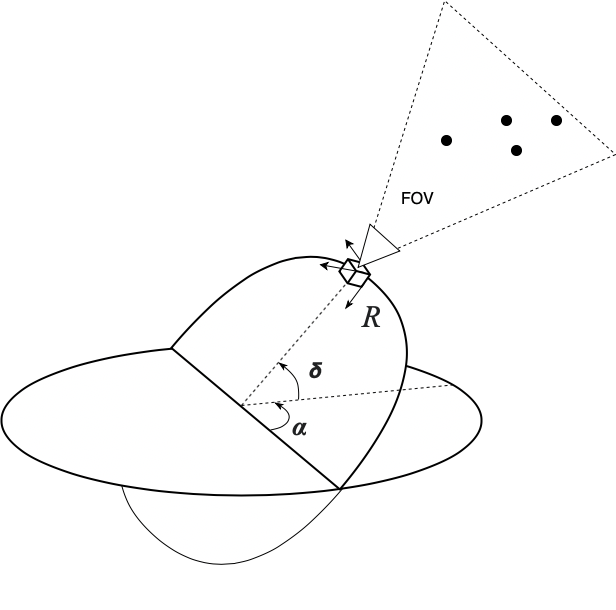
\includegraphics[scale=0.4]{figures/st_ref.png}
    \caption{Diagram of star tracker equipped satellite in orbit. Attitude and position elements are described by following symbols; \textbf{$\alpha$} being the right ascension, \textbf{$\delta$} declination and \textit{R} the attitude matrix. The star tracker camera system is visualized with four stars in the field of view (FOV).}
    \label{fig:orbit}
\end{figure}

A star tracker is an instrument that provides navigational data, such as position and attitude, by recognizing stars from optical images. The system consists of a camera and a computer. The system operates by capturing an image, processing it, and then comparing the extracted data to a star catalog. The star catalog contains columns of information about known stars. \citep{SatDesgin}
\par
Star tracker systems depend on image processing and analysis that run on varying computing platforms. The platform and purpose of the star tracker in focus is an FPGA-based star tracker for spacecraft attitude determination. The general idea of star tracker based attitude determination is explored in this chapter to explain the context of a pre-processing pipeline for such a system.

%The two-line element set is used for encoding the information about earth-orbiting objects. The two-line element of a satellite is used by ground stations or other satellites to estimate and predict the satellite position. 
%\par

%%%%%
%Any orbit of an object in space can be described by its six Keplerian orbital elements. The position of a satellite with a known orbit can be described by a function of the orbital elements and time. Five of the elements contribute to size, shape, and orientation of the orbit. The sixth element allows for calculation of the satellite position at a given moment in time. The two-line element set is used for encoding the information about earth-orbiting objects. The two-line element of a satellite is used by ground stations or other satellites to estimate and predict the satellite position. 
%\par
%The position of a satellite can also be described using the equatorial coordinate system. This  
%When a satellite is in earth orbit, the equatorial coordinate system is used for describing the position in relation to the earth. 
%\par
%The attitude of a spacecraft describes the way it is oriented in space, without taking into account movement or position. An attitude reference frame is used for representing the spacecraft attitude. The attitude reference frame may or may not be the same as the reference frame for the satellite orbit.
%\par
%Satellites in low-earth orbit can use onboard GPS, to accurately and reliably determine the position. A star tracker can then be used to reinforce the estimate of position and attitude. In deep space missions, the star tracker can be used together with passive radar systems to determine the position and attitude.

\section{Argumentation}
There are multiple ways to determine the position and attitude of a spacecraft. When the accuracy of the attitude needs to be better than $0.1{^\circ}$, a star tracker is to be used. When the high accuracy of a star tracker is not needed, other methods, such as navigation satellite systems or momentum wheels, can be used for determining the attitude and position. Often, however, a star tracker is used in combination with other attitude and position determination systems to reinforce the estimates.
\par
Other than accuracy advantages, the star tracker is also more independent than navigation satellite systems and mechanically simpler than momentum wheels. On the other hand, star trackers require more complexity in a computational sense. \citep{SatDesgin}
\par
A unique feature of star trackers is the ability to find the attitude and position of a spacecraft without any previous knowledge, also known as Lost-In-Space attitude determination. Momentum wheel-based navigation, for example, requires a reference to a previous position to determine its current position. The Lost-In-Space feature is also available using navigation satellite systems, although with limited range. \citep{SatDesgin}

\section{Image acquisition}
Images are usually captured by a charged-coupled device, or CCD, sensor. In contrast to another common image sensor type, the complementary metal-oxide-semiconductor (CMOS) sensor, CCD is more resistant to noise, resulting in higher quality images.
\citep*{SatDesgin}
\par
Star tracker cameras use a fixed focal length lens and a large field of view (FOV) to capture as many stars in the image as possible. A large FOV camera system consists of a large image sensor and a lens with small focal length. To maximize the brightness of the stars, the lens is equipped with a wide aperture for allowing more light to enter the image sensor. The camera system FOV is visualized in Figure \ref*{fig:orbit}. \citep*{SatDesgin}
\par
Star tracker camera sensors generally use the visible light spectrum to capture images. The images are stored in single channel, or black and white, format. Any color information is useless in star trackers, which benefit from high contrast and brightness of image features. This makes the image features more likely to be extracted and used for star detection. \citep*{SatDesgin}
\par
Star trackers in low-earth orbit satellites are faced with challenges due to the moon, earth, and sun. Images containing these objects are often overexposed, and unusable for the star tracker. To overcome these problems, a satellite can be fitted with two cameras, oriented 90\textdegree\ apart. Another option is to mount the camera on a side facing away from bright objects, and maneuvering the spacecraft to maintain the orientation. Other objects such as nearby satellites can also cause overexposure. The effect of these type of objects is less predictable, making it more difficult to mitigate the problems caused by them. \citep*{SatDesgin}

\section{Image processing}
The image processor of a star tracker extracts data from the captured image to use for star detection. The extracted data and processing algorithms vary between implementations, but the general idea is that the extraction process enhances the image features, scans the image for targets, and stores information about the targets for star detection.
\par
At the image processing stage, issues such as overexposed images and false star extractions are encountered. In the worst case, this leads to halting the star tracker, losing the currently prepared attitude and position update. In the best case, the issue can be corrected and the currently prepared update can be resumed.   
\par
The ideal output of the image processing is to have at least four bright stars extracted from the background. Using the relative position of each extracted star, the star tracker system is able to proceed to star detection. The image data is only used up to this stage, making it unnecessary from this point forward.

\section{Star detection}
The identification of stars is generally carried out by comparing identifiers, consisting of multiple stars. The identifiers are created by calculating the angular separation between bright stars found in the image. The angular separation can be determined relatively easily with a fixed FOV camera. \citep*{SatDesgin}
\par
The angular separation between any two stars is generally a unique identifier. This makes the process of star detection essentially a look-up operation, where known angular separations are compared against the identifiers created from the captured image. \citep*{SatDesgin}
\par
Four stars are used for creating the identifiers. The first two can be used as unit vector, while the third is required to resolve ambiguity. A fourth star is required for positive identification. \citep*{SatDesgin} \citep*{StreakDet}
\par
Given a set of recognized stars, or identifiers, the attitude and position can be calculated. The error detection and correction in this step is crucial, but somewhat easier than up to this point. False positives, as in stars that are mistakenly recognized, can be voted out when multiple stars have been matched. False positives are recognized by verifying their position in relation to other recognized stars. False negatives are more difficult to detect, and not a problem as long as there are enough recognized stars.

\section{Attitude and position}
The attitude and position are determined based on the recognized stars. With the known coordinates of the stars, the position and attitude of the satellite are calculated with the help of linear algebra. Finding the attitude can be generalized to solving the Wahba problem, where a rotation matrix between two coordinate systems is sought. By solving this problem, for example with singular value decomposition, the attitude matrix of the satellite can be obtained. To maximize the accuracy of the attitude estimation, the stars in the largest identifiers in the image are used for the matrix calculations. \citep*{StRef} \citep*{StreakDet}
\par
The position of the satellite can be estimated using trigonometric calculations using the recognized stars. The known positions and separation angles of the stars, together with the camera system FOV parameters, enable the satellite position to be calculated in relation to the stars. The position estimation is also reinforced with the help of multiple results. \citep*{StDev}

\chapter{Pre-processing pipeline documentation}

The goal of the documentation of the pre-processing pipeline is to explain the features and technical details of the implemented system. Each feature contributes to filling the requirements stated in the system specification. Figure \ref{fig:overview} shows an overview of the final product which includes the required components.

\begin{figure}[h]
    \centering
    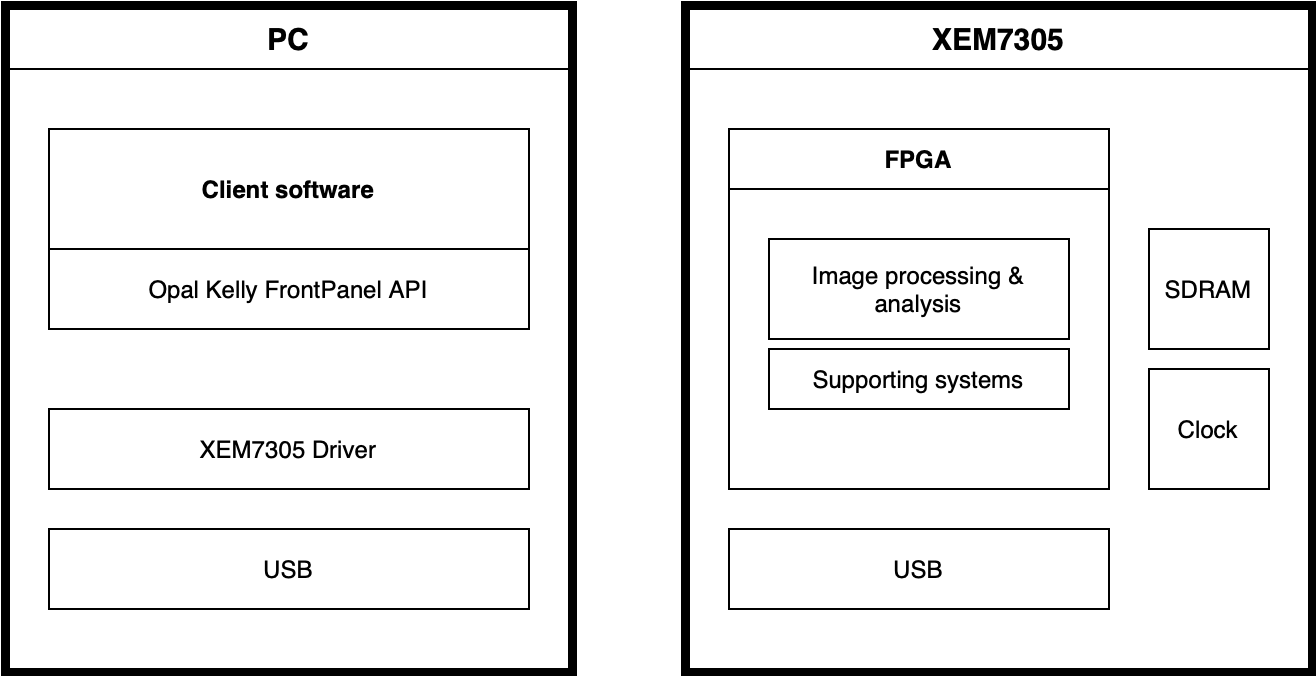
\includegraphics[scale=0.3]{figures/overview.png}
    \caption{Diagram of star tracker pre-processing pipeline. The FPGA, performing the image processing and analysis, on the right and the PC, being the user interface, on the left.}
    \label{fig:overview}
\end{figure}
% explain what is part of the onboard system 

\section{Functional overview}
The star tracker pre-processing pipeline is a system that uses an input image to extract features from. The features, in this case stars, can be used for further implementation of a star tracker. % how?
\par
The system can be integrated to a completely embedded environment, where it does not depend on a user interfacing client. 
An integration to a star tracker can be independent and highly isolated, with minor adjustments made to the off-chip module interfaces. Only a few essential parameters, triggers, and data are required.  
\par
From a user experience point of view, the pre-processing pipeline works by powering on the FPGA, then connecting it to the pre-processing pipeline client. The client then programs the FPGA with the pre-processing pipeline FPGA design. After successfully programming the FPGA, the pre-processing pipeline is configured with a valid image and parameters. The FPGA executes the image processing and analysis after which the client reads the result, consisting of an image and metadata, for the user to evaluate.
\par
From an integrated system point of view, the pre-processing pipeline is powered on and configured by an external system, for example, a program on a microprocessor. The external system has the same control and responsibility as the client software. To make the integrated system autonomous, a more sophisticated parameter tuning is needed for the pre-processing pipeline to be effective. This is desirable when integrating a system to a spacecraft, since it often requires a high degree of autonomy.

\section{FPGA design}
The FPGA design is modeled with Verilog HDL. Xilinx Vivado design suite is used for generating bitstream files that are programmed to the Opal Kelly XEM7305 FPGA module.
\par
The star tracker pre-processing pipeline FPGA design contributes to all system requirements in Table \ref*{table:sysreq}. The requirements are satisfied by combining a set of components. Some components contribute to several requirements, while others are less multipurpose. Figure \ref*{fig:fpga_design} shows an overview of the components in the design.

\begin{figure}[h]
    \centering
    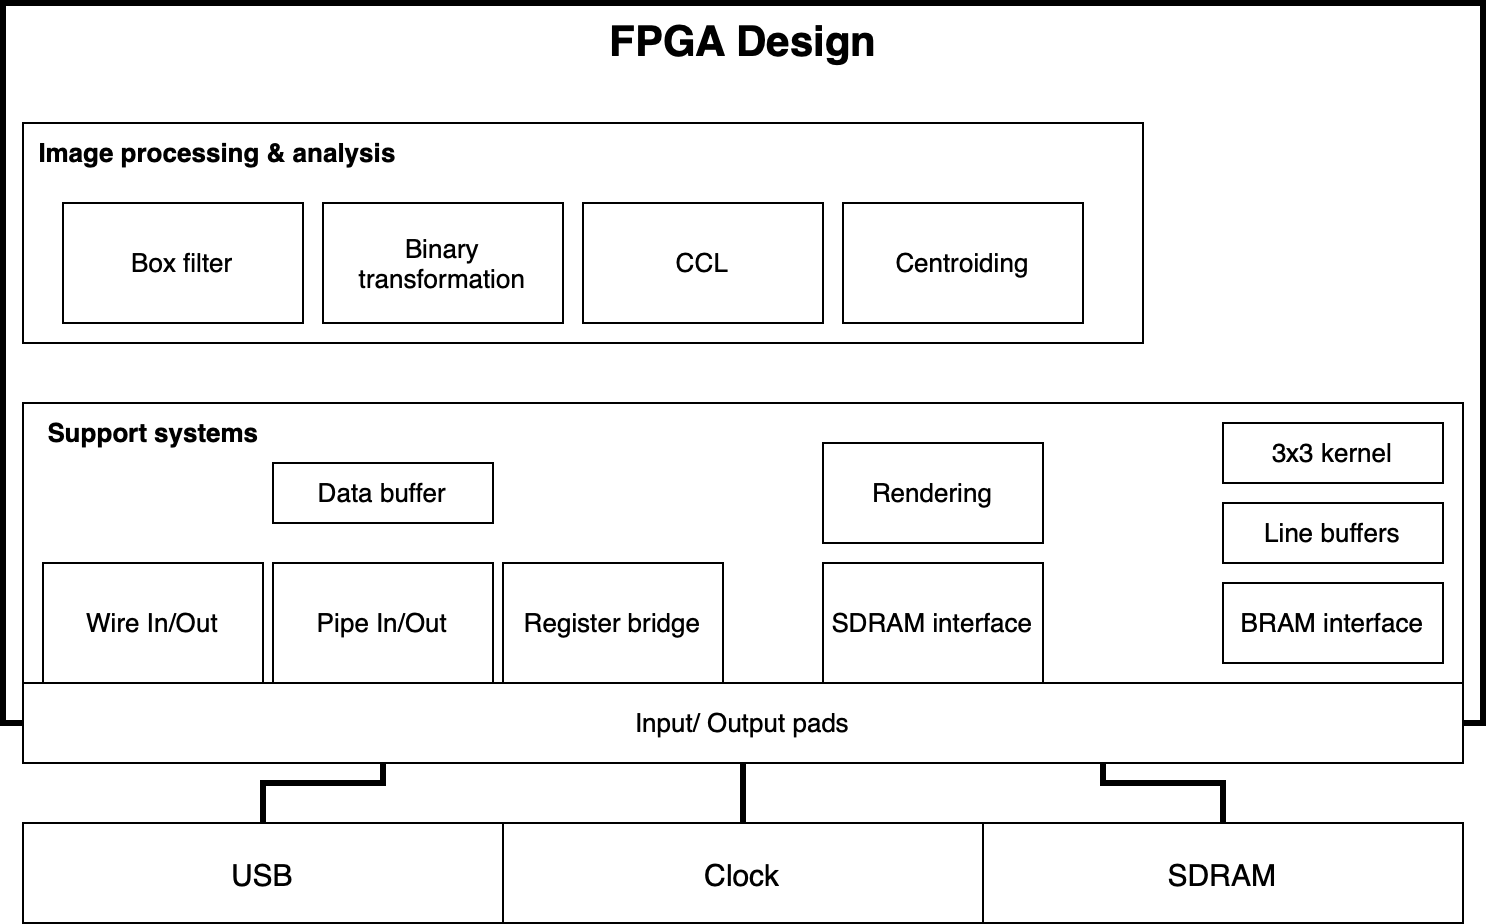
\includegraphics[scale=0.25]{figures/fpga_design.png}
    \caption{Diagram showing FPGA design as functional blocks where top section is furthest from off-chip modules while bottom section is closest to off-chip modules. Boxes in the diagram are not in scale to the actual footprint of the components on the FPGA.}
    \label{fig:fpga_design}
\end{figure}

\subsection{Support systems}
The supporting systems included in the FPGA design consist of components that do not contribute to image processing and analysis directly, but provide other necessary features, such as storage and communication. 
\par
The core supporting systems of the FPGA design consist of modules provided by Opal Kelly. These include communication, buffering, and storage solutions that are specific to the FPGA and off-chip components. \citep{stpp}
\par
The bottom section of Figure \ref*{fig:fpga_design} shows the main functional components of the support systems in the FPGA design. The isolation of this section can be made in a functional, and in some cases, technical sense.

\subsubsection{Communication and host interface}
The Opal Kelly host interface, called okHost, is a gateway for controlling and monitoring the FPGA. It contains the logic for communication with the FX3 USB microcontroller, exposing signal endpoints for controlling USB communication. The host interface also contains a clock signal derived from the external clock module on the XEM7305 board. The 100.8 MHz clock signal synchronizes the logic in the FPGA design with the USB microcontroller operations. \citep{XEM7305Man} \citep{FrontPanelMan} \citep{stpp}
\par
Opal Kelly provides a set of IP core modules supporting data transfer from single bits to megabytes. Different synchronization and control methods are used for each module, resulting in small scale data transfers being simpler than large scale transfers. Three Opal Kelly communication modules are used within the FPGA design, each with its own purpose.
\par
The Opal Kelly register bridge connects the host interface directly to a dedicated address space on the FPGA. The register bridge is connected to a 32-bit wide address bus, with 32 bits of storage for each address to use synchronously. The register bridge interface contains separate 32-bit data buses for input and output, and a register address bus. This adds complexity to the FPGA design, because a mapping mechanism, for example a multiplexer, is needed to make all 32 addresses usable. The register bridge is used through the Opal Kelly API, in the client software. Figure \ref*{fig:fpga_design} shows the register bridge connected to the input/output pads, which act as interface between the register bridge and the off-chip modules. The required off-chip modules for the register bridge are clock and USB. \citep{FrontPanelMan} \citep{stpp}
\par
Wire In and Wire Out modules are directional 32-bit buses that transfer data asynchronously. The Wire In/Out modules are by their asynchronous nature, and limited capacity, good for state management and triggering events. The asynchronous data are nevertheless, in many cases, synchronized to a clock in the design. Figure \ref*{fig:fpga_design} shows the Wire In/Out connected to the input/output pads, giving them access to the USB off-chip module. \citep{FrontPanelMan} \citep{stpp}
\par
Pipe In and Pipe Out modules are used for multibyte synchronous data transfer. The data buses on both modules are 32 bit wide. The block throttled variant of the modules adds negotiation signals to the communication system, which allows the FPGA to control the flow of data. The PC can initiate the data transfer, but unless the \verb|EP_READY| control signal is high, data are not sent. This is useful in cases where incoming data needs to be stored using buffers. Figure \ref*{fig:fpga_design} shows the Pipe In/Out connected to the input/output pads, allowing it to interface with clock and USB off-chip modules. \citep{FrontPanelMan} \citep{stpp}
% define block throttled variant
% define high signal
% define states and events, example
\subsubsection{FPGA state management and event triggers}
The Wire In module is used on the FPGA to enter states that need to be externally managed. Table \ref{table:wireInState} shows a description and wire values of them. The Wire In uses only the first four bits of the 32-bit data and the values are set so that only one state can occur at a given moment, which ensures the predictability of the system. Each state in Table \ref*{table:wireInState} is mapped to an index, which is used to read the value corresponding to the state on the 32-bit Wire In data bus. \citep{stpp}
\par
The Wire Out module has the single purpose of providing verification of the setup of the FPGA. The signal is expected to be high after a small delay after the FPGA is powered on and the bitstream is programmed. Table \ref*{table:wireOutState} shows the description and wire value of the Wire Out state. \citep{stpp}

\begin{table}[h]
    \begin{tabular}{|p{3cm}|p{10cm}|}
        \hline
        \textbf{Wire value}&\textbf{Description}\\
        \hline
        0x0001&Read storage to Pipe Out. Used when reading image back from the FPGA to the client.\\
        \hline
        0x0002&Write to storage from Pipe In. Used when writing an image from the client to the FPGA.\\ 
        \hline
        0x0004&Resets FIFO buffers. Used between image reads and writes. \\
        \hline
        0x0008&Triggers image processing and analysis. Used when the FPGA is configured and ready to perform star extraction.\\
        \hline
    \end{tabular}
    \caption{Description of Wire In state control bits.}
    \label{table:wireInState}
\end{table}
\begin{table}[h]
    \begin{tabular}{|p{3cm}|p{10cm}|}
        \hline
        \textbf{Wire value}&\textbf{Description}\\
        \hline
        0x0001&Memory calibration signal. Used to verify successful initialization of the SDRAM memory.\\
        \hline
    \end{tabular}
    \caption{Description of Wire Out state bits.}
    \label{table:wireOutState}
\end{table}

The Wire In/Out modules are a good suit for the state triggers because of the reactive and simple user experience.
The state management and event trigger system contributes to satisfying the system requirements. The features provided by the Wire In module are fundamental to the requirements \hyperref[req1.3]{1.3}, \hyperref[req1.4]{1.4}, \hyperref[req2.2]{2.2}, and \hyperref[req3.3]{3.3}.

\subsubsection{Parameter configuration and metrics}
To allow data transfer for accessing register values on the FPGA, the Opal Kelly register bridge is used. The registers are addressed so that the first 15 contain writable data, and the second 15 contain readable data. This prevents any concurrency issues with register access. Pre-assigned values to the writable addresses ensure that the pre-processing pipeline parameters have default values to use in case none are assigned through the register bridge. Tables \ref{table:regs1} and \ref{table:regs2} explain the use of the register bridge. \citep{stpp}
\par
The features enabled by the register bridge for parameter configuration and metrics contribute to system requirements \hyperref[req1.2]{1.2}, \hyperref[req1.3]{1.3}, \hyperref[req1.4]{1.4}, \hyperref[req2.2]{2.2}, and \hyperref[req3.3]{3.3}.

\begin{table}[h]
    \begin{tabular}{|p{2cm}|p{2cm}|p{9cm}|}
        \hline
        \textbf{Address}&\textbf{Data}&\textbf{Description}\\
        \hline
        0x0000&32-bit int&Minimum brightness of an image feature. Used to filter out faint objects in the image.\\
        \hline
        0x0001&8-bit int&Binary transformation threshold. Used for filtering faint pixels out when preparing image for feature detection.\\ 
        \hline
    \end{tabular}
    \caption{Description of writable values used by the FPGA.}
    \label{table:regs1}
\end{table}
% Explain tables in text
\begin{table}[h]
    \begin{tabular}{|p{2cm}|p{2cm}|p{9cm}|}
        \hline
        \textbf{Address}&\textbf{Data}&\textbf{Description}\\
        \hline
        0x000F&32-bit int&Image processing and analysis timer. Used for evaluating performance. Stored in register as clock cycle count.\\
        \hline
        0x0010&32-bit int&Box filter timer. Used for evaluating box filter algorithm performance.\\ 
        \hline
        0x0011&32-bit int&CCL timer. Used for evaluating CCL algorithm performance.\\
        \hline
        0x0012&32-bit int&Feature rendering timer. Used for evaluating performance of feature rendering.\\
        \hline
    \end{tabular}
    \caption{Description of readable registers on the FPGA.}
    \label{table:regs2}
\end{table}

\subsubsection{Image transfer and SDRAM storage}
The size and format of the pre-processing pipeline input image require some mechanisms to be implemented to allow transfer and storage of the image data. The image is fixed as to size and format, namely 270 x 480 pixels, single channel, and eight bits per pixel. The image is not compressed to decrease image processing complexity, making the total image size 129.6 kb.
\par
The Pipe In module is used to receive the image data on the FPGA. The module is connected to, and partly managed, by a FIFO buffer. The buffer is also connected to the SDRAM interface, which pulls data from the buffer to storage. The entire data flow is thus controlled by the SDRAM, which is the bottleneck of the image transfer system. \citep{stpp}
\par
The 32-bit wide data bus of the Pipe In module is connected to the input of the FIFO buffer. The buffer capacity is 128 bits to suit the input data bus width of the SDRAM interface. Both Pipe In and FIFO modules are synchronized to the host interface clock. The SDRAM interface is synchronized to its own 87 MHz clock, also derived from the 200 MHz system clock. The modules are synchronized together with control signals to manage the data flow and to mitigate any issue with clock speed differences. \citep{stpp}
\par
Beyond the input image, the SDRAM is used to store intermediate image processing results. The sequential process writes an image to storage after each step. Since each output is only needed as the input to the next step, the stored images can be overwritten. The process requires a storage capacity of three times the image size, one of the images being the original. The original image is kept in case the process is to be re-executed. In an integrated environment, the storage capacity could be scaled down to two times the image size, since the original image would be useless. \citep{stpp} % why?
\par
After image processing and analysis the output image is stored to SDRAM. The output image is transferred from SDRAM to an external endpoint using the Pipe Out module through another FIFO buffer. The image output transfer uses a similar FIFO buffer as the input image transfer, except with reversed port widths and other control signals. \citep{stpp}
\par
The image transfer and storage systems contribute to system requirements \hyperref[req1.4]{1.4} and \hyperref[req2.2]{2.2}.

\subsubsection{Line buffer and BRAM storage}
The image data are accessed by the image processing and analysis components through line buffers implemented as BRAM. Each line consists of 270 8-bit pixels, and three lines are stored in the buffer. This geometry enables image processing on both the horizontal and vertical axis of the image. Figure \ref*{fig:mem_overview} shows the line buffer in the middle, as the intermediate storage mechanism. \citep{stpp}
\par
The dual port BRAM has two data buses and two address ports to allow simultaneous read and write operations. The interface also includes a 270-bit data mask to select which pixels to write to BRAM. This adds complexity to the line buffer system but reduces the number of registers needed. \citep{stpp}
\par
The line buffer system is the intermediate storage between the image storage and image processing. The read and write operations are triggered by counters that are updated during the image processing. The line buffer is filled by initiating a read operation to the SDRAM. After each burst read, 128 bits of data are pushed to the buffer and the SDRAM read address is updated. The read address is incremented by 8 between reads, since the burst mode of the SDRAM covers 8 addresses. The SDRAM read continues until the buffer is full. \citep{stpp}
\par
The line buffer can be seen as a sliding window on horizontal axis of the image. The buffer, and image processing, is initialized by filling all three buffers. While processing the image, one line after another is read into the buffer. The image columns are mapped to BRAM using addresses and indices. The indices track which address points to which column, while the addresses are fixed variables to point to the start of an image column in BRAM. The addresses are rotated between the indices to predictably and efficiently use the BRAM address space. \citep{stpp}
\par
A big portion of the logic in the pre-processing pipeline is for moving around image data, making the line buffers a core part of the support systems, and storage mechanisms in the FPGA design. The line buffers contribute to system requirements \hyperref[req2.2]{2.2}, \hyperref[req3.1]{3.1}, and \hyperref[req3.2]{3.2}.

\begin{figure}[h]
    \centering
    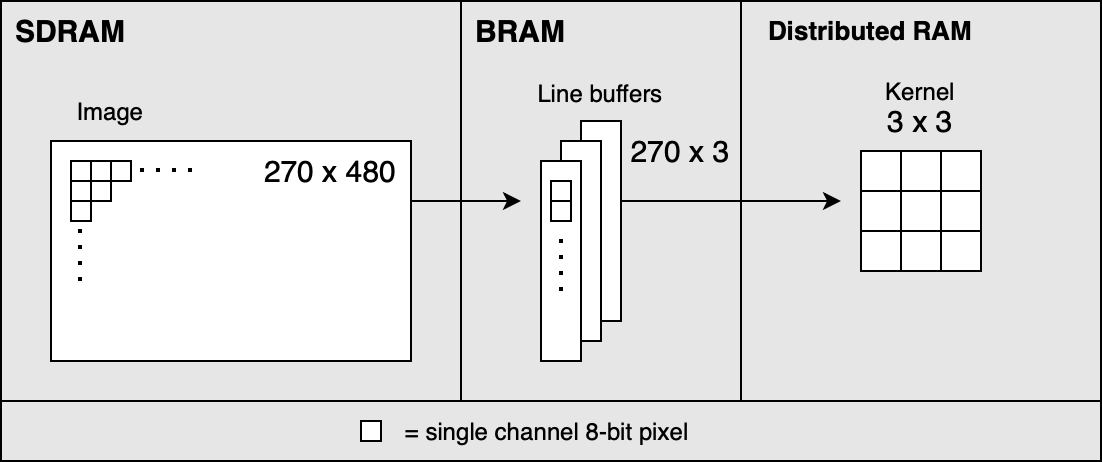
\includegraphics[scale=0.3]{figures/mem_overview.png}
    \caption{Diagram of different levels of memory used for storing image pixels of the star tracker pre-processing pipeline.}
    \label{fig:mem_overview}
\end{figure}

\subsubsection{3x3 Kernel}
The lowest level storage mechanism where image pixels are kept are three small line buffers, forming a 3 x 3 pixel sliding window, or image processing kernel. It is implemented in distributed memory, within the FPGA fabric. The kernel consists of three pixels from each column in the line buffer, creating the 3 x 3 pixel geometry shown in Figure \ref*{fig:mem_overview}. Data from the line buffer is fed into the kernel data structure which is then used for image processing and analysis. The results of these operations are written directly to a higher level storage. Thus the data flow is directional within this storage mechanism. \citep{stpp}
\par
Between each processed pixel, the kernel moves one step. This movement consists of three read operations from BRAM to the kernel, each line buffer contributing with three pixels. The entire kernel is overwritten each time, since the data transfer is relatively low. \citep{stpp}
\par
The image processing kernel contributes to system requirements \hyperref[req2.2]{2.2}, \hyperref[req3.1]{3.1}, and \hyperref[req3.2]{3.2}.

\subsubsection{Rendering}
The rendering process creates an image output from the data generated within image processing and analysis. The data generated from star extraction in the pre-processing pipeline is stored in tables and buffers for convenience. Rendering an image with this data provides visual feedback of the process.
\par
Rendering relies on the kernel and line buffers to write the image data to SDRAM. The image is rendered in the original 270 x 480 single channel 8-bit format to SDRAM between the image processing steps, and for final output. The rendering process contributes to system requirement \hyperref[req2.2]{2.2}. \citep{stpp}

\subsection{Image processing and analysis}
To extract stars from an image, a number of image processing algorithms are implemented. The general idea is that an image containing bright stars in the foreground and faint objects or empty space in the background is used as input. The first algorithm smoothens the image to create larger and more detectable foreground features. The second process separates the foreground from the background with a threshold. This is to enable connected component labeling (CCL) in the next step, which requires a fully separate foreground and background. The connected component labeling algorithm traverses through the image pixels and assigns them to features. Metrics of the features are stored for calculating the centroid in the final step. \citep{stpp}
\par
As a core part of the pre-processing pipeline, the image processing and analysis contribute to all system requirements in Table \ref*{table:sysreq}.

\subsubsection{Box Filter}
A box filter is applied on the image to prepare the image for CCL. The principle of the box filter is to expand and blur features in the image by replacing a pixel with the average of the surrounding pixels. The 3 x 3 kernel is used for this filter, where the center pixel is the target. This filter is commonly described by the expression 
 
$x_{ij}=\frac{1}{9}
\begin{bmatrix}
1 & 1 & 1\\
1 & 1 & 1\\
1 & 1 & 1
\end{bmatrix}
$,
where $x$ is the currently updated, center pixel in the kernel. The matrix represents the kernel with pixel values. This gives a uniformly applied average of the image where high value pixel areas are expanded without too much loss of detail. Figure \ref*{fig:box_filter} shows an example of a feature passing through the box filter. The blurring and expansion of the feature are apparent. \citep{stpp}
\par
% https://en.wikipedia.org/wiki/Division_algorithm
A problem with the box filter is the need for integer division. A division operation is problematic when implemented in hardware and is often dedicated a separate IP core module. This increased complexity can, however, be avoided in the case of the box filter because it lacks the need for high accuracy output of the operation, as the pixel values are 8-bit integers. The alternative operation to replace the division takes advantage of the constants in the box filter, which are the output bit width and the denominator. The lack of accuracy is compensated by the performance which is reduced from a multi clock cycle operation to a single clock cycle operation. The division is approximated with the expression
$
(\sum x_{ij} \cdot 28) \gg 8 
$, where $x$ is the 3 x 3 kernel. The theoretical accuracy of the approximation is 98 \%. In practice this depends on the value of $\sum x_{ij}$. \citep{stpp}
\par
Image edges are handled by ignoring the pixel value and setting them to 0. This assigns the edges of the image as part of the background feature. The possible loss of edge features is also acceptable because of the difficulty to approximate the complete geometry and center of an edge feature. \citep{stpp}

\begin{figure}[h]
    \centering
    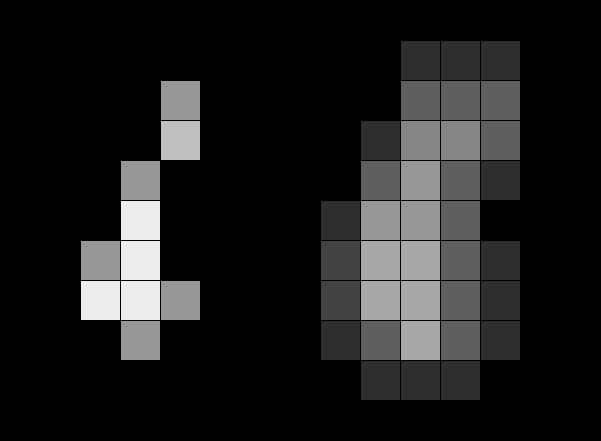
\includegraphics[scale=0.25]{figures/box_filter.png}
    \caption{Illustration of box filter. The original feature is on the left, while the processed feature is on the right. Box filter averages every pixel within a 3 x 3 image processing kernel.}
    \label{fig:box_filter}
\end{figure}

\subsubsection{Thresholding}
Thresholding is done to separate the background from the foreground in the image. The foreground needs to contain enough pixels to enable successful star extraction. The box filter allows foreground feature edges to be brighter, which otherwise might be categorized as background in this step. If the threshold is too low, background and noise blend together with foreground features, making the choice of optimal threshold a complex problem. This is out of scope of this project and the threshold is manually set.
\par
An example solution for setting the threshold could be to use a feedback loop to adjust the parameter. The loop would use previous output of the pipeline to use as input, providing the number of stars, brightness, and distance to determine a threshold setting and acceptable result.
\par
The thresholding process transforms each pixel value to either 0, being background, or 255 as foreground. Figure \ref*{fig:thresholding} shows an example of the thresholding process. The example shows most of the original pixels passing the threshold. These are assigned to foreground, with the value 255. Some pixels around the edges are too faint to pass the threshold. These pixels are assigned to background with the value 0. \citep{stpp}
\par
 As this is a process with no dependency on neighboring pixels, it can be conveniently placed in the output phase of the box filter. The output phase is where the result of the box filter operation is written to SDRAM memory. The register containing the output of the box filter is piped to the SDRAM write bus through the threshold. This makes the thresholding highly efficient because of no additional clock cycles required. \citep{stpp}

\begin{figure}[h]
    \centering
    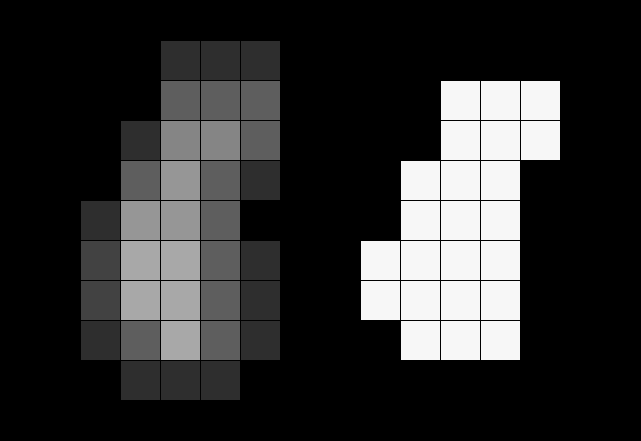
\includegraphics[scale=0.25]{figures/thresholding.png}
    \caption{Illustration of thresholding process. The feature on the left is the product of box filter, and the feature on the right is the feature after passing the threshold.}
    \label{fig:thresholding}
\end{figure}

\subsubsection{Connected component labeling and analysis}
The goal with CCL is to assign foreground pixels to features. The algorithm traverses the image using a kernel, updating the feature tables and pixels in the line buffer. Three feature tables keep information about pixel values and the feature geometry. Figure \ref*{fig:feature_tables} shows the three tables, populated with example data.
\par
Every encountered foreground pixel is updated depending on its neighbors. The focus is on the center pixel in the kernel. It is updated depending on the neighboring pixels. If any neighboring pixel has a value with an entry in the feature table, the current pixel is updated and mapped to the same feature. The geometry of each feature is stored as minimum and maximum coordinates within the image. Also the brightness of each feature is stored. This is used together with the geometry for feature analysis. \citep{stpp}
\par
The requirement for a component to be connected to a feature is that at least one side of the pixel touches the feature, making it a 4-connected feature. In contrast, an 8-connected feature accepts diagonally connected components. Diagonally connected components are not detected in this CCL implementation because the previously performed box filtering already exaggerates the component connections, filling the gaps between pixels. \citep{stpp}
\par
The 4-connect comparison is done by comparing the top center and left center to the center pixel in the kernel. The movement of the kernel mitigates the need for comparing all four connections surrounding the center pixel in the kernel. This simplifies the design while keeping the line buffer mechanism uniform with the other parts of image processing. \citep{stpp}
\par
Conflicts in the feature table are encountered when connected components refer to multiple features. This happens when the shape of the feature is unfavorable in regard to kernel movement and the component comparison process. A conflict is resolved by merging the connected features. This is done by merging the brightness of the features involved, updating the feature coordinates, and reassigning the feature label. Depending on the number of mergers, a single feature might be mapped to a number of pixel values. Figure \ref*{fig:feature_tables} shows an example of a resolved conflict, where pixel values \textbf{0x04} and \textbf{0x05} are mapped to the same feature, \textbf{0x03}. \citep{stpp}
\par
While traversing the image, CCL will enter one of three states for each foreground pixel, while background pixels are ignored. When encountering a foreground pixel in the left center, it can be assumed to belong to a feature. The state where left center is foreground is prioritized, because the feature it refers to has the earliest entry in the feature table. The feature with the earliest entry needs to be selected in order for the center pixel to avoid conflicts. The next priority is to compare the top center pixel. This state updates the center pixel with the value of the top pixel. A new feature is created when neither the left center or top center pixel is in the foreground. This state adds an entry to the feature tables. \citep{stpp}
\par
The implemented CCL algorithm is streamlined and simple, but not without drawbacks. The most significant limitation is the number of features that can be stored. In case all foreground features in the image are square, the maximum number of features is 253. This is more than enough for what a star tracker needs, but depending on the number of conflicts the number of available features is significantly lower. This limitation originates from the 8-bit pixel values stored in the feature tables and the lack of re-renders of the CCL image. With re-rendering implemented, the maximum would be guaranteed to be 253 features, instead of 253 as best case. The trade-off for choosing re-render to allow for more features would be a performance loss and a larger memory and FPGA design footprint. \citep{stpp}

\begin{figure}[h]
    \centering
    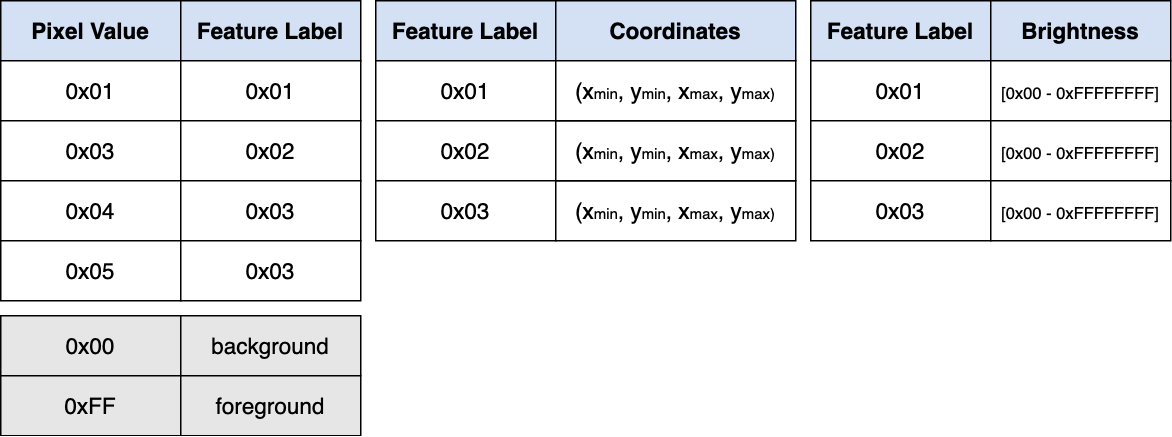
\includegraphics[scale=0.35]{figures/feature_tables.png}
    \caption{Example of CCL feature tables. Left table is where the mapping of pixel values to feature labels is stored. Labels are also renderable, as they are stored as 8-bit integers. Center table stores minimum and maximum coordinates of each feature in 35-bit integers. Right table stores feature brightness as 32-bit integers.}
    \label{fig:feature_tables}
\end{figure}

\subsubsection{Feature detection and centroiding}
Feature detection is the process of using the feature tables, shown in Figure \ref*{fig:feature_tables}, to create image data to indicate detected features. Centroiding gives a more accurate indicator of the detected features by further analyzing them. Feature detection and centroiding are the final step of the pre-processing pipeline, resulting in an output image and data points for the extracted stars. 
\par
The feature detection process filters out features that are too faint or small. The threshold is specified by the parameter configuration system. Table \ref*{table:regs1} shows the register and format of the threshold. The threshold is compared with the brightness of each feature, which is calculated in the CCL process. An example of the feature brightness table is shown in Figure \ref*{fig:feature_tables} on the right. When the brightness of a feature is below the threshold, it is discarded. The process then moves on to validate the next feature in the feature table. \citep{stpp}
\par
Unlike other parts of the image processing and analysis, feature detection traverses the image one feature at a time. The sliding window favors processing that needs to scan the entire image, possibly applying calculations to every pixel. Feature detection is only interested in processing known coordinates of the image, making the sliding window unfavorable. \citep{stpp}
\par
A rectangle can be imagined around a feature, given the maximum and minimum coordinates of it. The pixels within this rectangle are read directly from SDRAM to the feature detection process. This bypasses the commonly used sequential SDRAM read procedure. A more complex addressing scheme is required to obtain the correct pixels. Due to the SDRAM burst mode, the correct address needs to take into account both pixel location and burst read suitability. Then an offset value is calculated to access the correct value in the SDRAM read buffer. \citep{stpp}
\par
The commonly used SDRAM write procedure is also bypassed by the feature detection process. The addressing scheme used for reading the feature pixels is also used for writing them back. The data mask in the SDRAM interface is used by this process to simplify the data flow. It ensures that only a selected part of the write buffer is written into SDRAM. Since the number of pixels updated by this process is relatively low, the absence of a data mask would result in the need of copying the read buffer, only for most of it to be copied back to the write buffer. The configuration of the data mask is relatively simple since the pixel offset is already calculated by the addressing scheme. \citep{stpp}
\par
Depending on the size of a feature, the pixel values are stored in registers. Centroid calculation is performed on features of suitable size. Suitability comes from the number of registers required for storing all pixel data of the feature. The pixel values for centroid calculation could be stored in BRAM to allow larger features to obtain a weighted centroid. \citep{stpp}
\par
A position estimate for every feature is calculated to achieve system requirements \hyperref[req3.1]{3.1} and \hyperref[req3.2]{3.2}. The centroid is calculated in one of two ways, a weighted and non-weighted version.
\par 
The weighted centroid of a feature estimates the true center of it. The process takes into account pixel brightness values and distance from the average coordinate. An average coordinate is the value between the minimum and maximum coordinates, stored in the feature table. The process creates an integer value for every row and column of the feature using these calculations. Each pixel in the feature contributes with its brightness, while the column or row number contributes with the weight. The calculation can be described with the following expression $C_{i} = C_{i} + \texttt{0xffff} - F_{jk}|i-c|$, where $C_{i}$ is the feature column register, \texttt{0xffff} is a constant for the weight, $F_{jk}$ is a pixel value, and $|i-c|$ is the distance from the average coordinate. \citep{stpp}
\par
A detail to notice in the weighted centroid calculation is the requirement of pixel brightness values. The image processing and analysis have until this point used the output of the previous step as input to the next step. The brightness data used for weighted centroid calculation comes from the output of the box filter. This image is used because the pixels have the same geometry as they have in the feature table, and contain pixel brightness information. \citep{stpp}
\par
The weighted centroid calculation results in column and row registers which are used to determine and render the estimated center of the feature. The coordinate of the center, relative to the feature, is the indices of the column and row registers with the highest values. \citep{stpp}
\par

\begin{figure}[h]
    \centering
    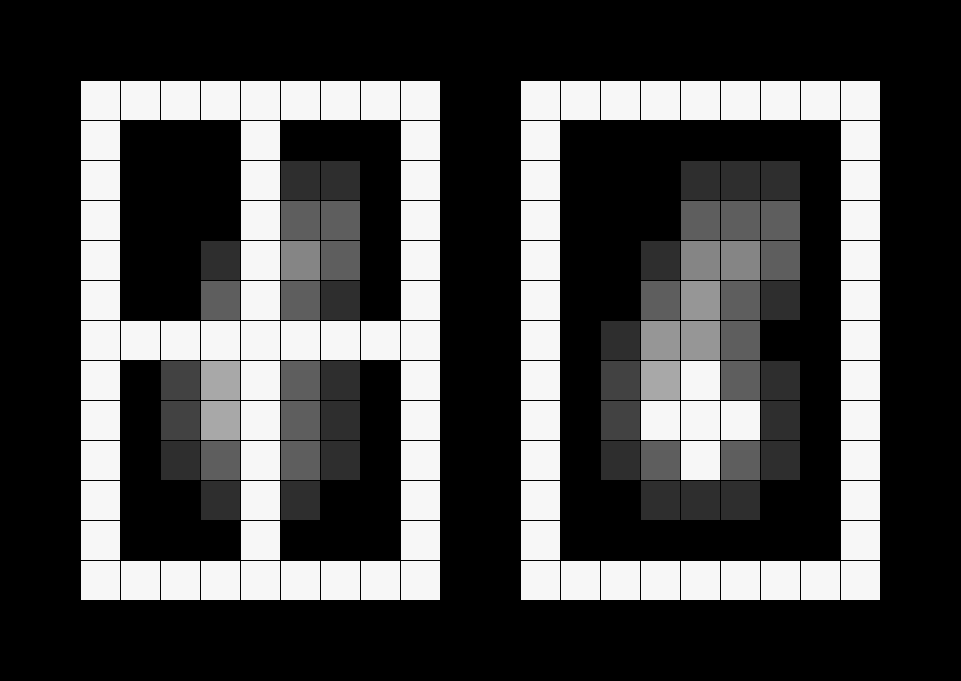
\includegraphics[scale=0.25]{figures/centroid.png}
    \caption{Illustration of the two centroid variants. Non-weighted centroid is rendered on the feature on the left. Weighted centroid is rendered on the feature on the right.}
    \label{fig:centroids}
\end{figure}

The non-weighted centroid calculation uses the minimum and maximum coordinates of each feature to calculate the average coordinate as the center. This estimation of a feature center is not as accurate as the weighted, but acts as fallback in case the weighted option is not suitable. \citep{stpp}
\par
Figure \ref*{fig:centroids} shows an example of the result of feature detection and centroiding. The detected features are rendered with a rectangular frame around the edges, with a small offset from the coordinates of the feature table, for better visibility. Both centroid variants are rendered as a cross on the corresponding feature. The non-weighted variant has a cross extending from the feature frame, while the cross of the weighted variant is significantly smaller. This helps with distinguishing the variants, and the visual analysis of the weighted centroid.

\section{Client endpoint}
The client endpoint is the external operator of the pre-processing pipeline and responsible for controlling the FPGA module. The features provided by the client endpoint contribute to system requirements \hyperref[req1.1]{1.1}, \hyperref[req1.2]{1.2}, \hyperref[req1.3]{1.3}, \hyperref[req1.4]{1.4}, and \hyperref[req2.2]{2.2}. The purpose of the client endpoint is to allow operation and development of the system. This is made easy by the use of Opal Kelly API, which makes controlling the FPGA module dynamic and simple. Optionally, the system could be more self-sustaining by handing over some client responsibilities to the FPGA module. A self-sustaining system might be ideal in an integrated system in production, but inconvenient for development and demonstration. \citep{stpp}
\par
The client endpoint is a Java-based PC application with a graphical user interface (GUI) that enables debugging, analysis, and parameter configuration. The application uses the JavaFx platform, making it lightweight and portable. \citep{stpp}
\par

\subsection{Connecting and initializing FPGA}
The base class, called \texttt{okCFrontPanel}, is the entry point for operating the FPGA module. It provides methods for device interaction, device configuration, and FPGA communication. The FPGA module is initialized by calling the API to open a connection. This enables the communication layers required for interacting with the FPGA module. \citep*{FrontPanelMan} \citep{stpp}
\par
Before programming the FPGA, the device is configured with a default configuration from on-chip flash memory, and checked for errors. When encountering errors, they are reported to the user, but no further action is taken. \citep{stpp}

\subsection{Bitsream programming}
The bitstream file, containing the FPGA design, is programmed to the FGPA using the \texttt{okCFrontPanel} class. To program a bitsream file to the FPGA, an open and initialized device is required. When encountering errors in the programming stage, these are reported to the user, and a reset signal is sent to the FPGA. The memory calibration is initiated on the FPGA as it is programmed. The test result is verified by reading the Wire Out value from the FPGA, shown in Table \ref*{table:wireOutState}. Errors encountered in this stage are simply reported to the user. \citep{stpp}

\subsection{Pre-processing pipeline configuration and control}
The configurable parameters and triggers are listed in Tables \ref*{table:wireInState} and \ref*{table:regs1}. To enable these features, a programmed device is required. \citep{stpp}
\par
The binary transformation threshold and feature brightness threshold are read from user input. The values are validated and written to the register bridge on the FPGA using the \texttt{okCFrontPanel} class. Any errors are reported to the user. \citep{stpp}
\par
To select an image for the pre-processing pipeline, it is first loaded to the client application. The 270 x 480 resolution, 8-bit single channel bitmap file format is used. The selected image can be viewed in the GUI, but this feature is most useful for analysis after executing the pre-processing pipeline. The image is prepared by converting it to a byte array of integers. This is the format required by the Pipe In module. The FPGA is prepared for image transfer by configuring its state with the Wire In values listed in Table \ref*{table:wireInState}, which resets the FIFO buffers and sets the SDRAM to read mode.
The write is then performed using the Block Pipe Out module, by calling the \texttt{okCFrontPanel} class. \citep{stpp}
\par
The pre-processing pipeline can be executed when the parameters and image are configured. The 
process is started by setting the Wire In value, as seen in Table \ref{table:wireInState}. This triggers the pre-processing pipeline on the FPGA. Error detection in this stage is difficult, and only detectable when the output image is viewed. \citep{stpp}

\subsection{Results and analysis}
The output image can be read from the FPGA when the pre-processing pipeline is completed. This is initiated in a similar manner as writing an image to the FPGA, except for the Wire In value. After the FIFO buffers and SDRAM are reset, the image is read to the client by the Block Pipe In module, provided by the \texttt{okCFrontPanel} class. The image is saved to disk, in the same format as the input image. \citep{stpp}
\par
The output image can be viewed after it is transferred from the FPGA-module to the client endpoint. Analysis of feature detection is made simple by having the input and output images side by side. The zoom and movement features enhance the user experience further. The detected stars are distinguished by the frame outline and centroid, as seen in Figure \ref*{fig:centroids}. \citep{stpp}

\chapter{Results and comparison}

%The output of the pre-processing pipeline consists of the metrics and data generated from input images. 

% The output of the pre-processing pipeline is the data generated by the system processing an image. User-friendly validation and verification of the success of the process is done using the client endpoint. The raw data, generated by each process in the pipeline, is used to rendered an image, which leads to it containing more information than the raw data separately. The output image is thus used for result analysis.

\section{Pre-processing pipeline results}
The results of the pre-processing pipeline are presented as four use cases. The standard procedure of the pre-processing pipeline is to use an input file together with input parameters to produce an output. Each use case contains two runs, each consisting of input parameters, output image, and metrics.  
\par
The data set consists of generated test data and image data from the StreakDet input dataset. The images from the Streakdet dataset are selected to highlight features of the pre-processing pipeline, such as thresholds and weighted centroiding.

\subsection*{Test input}
A test input, shown in Figure \ref{res:t_in}, is used to visualize the standard procedure of the pre-processing pipeline. The data is synthesized by gathering an overview of the StreakDet dataset and creating a layout of pixels that resembles commonly seen stars.
\par
To showcase weighted centroiding, the dimensions and pixel value gradient of the stars are taken into account. The gradient helps with visually verifying the process, since the centroid location becomes more obvious.
\par
Figure \ref{res:t0} shows the result when a foreground threshold of 50 and feature threshold of 300 are applied. All features are detected, and one gets a weighted centroid, seen in the top right corner. Feature \ref{res:t1} shows the result when increasing the foreground threshold to 100 and keeping the feature threshold at 300. Less pixels are assigned to foreground, making the features smaller. This enables more features to receive a weighted centroid. 

\begin{table}[h!]
    \centering
    \begin{tabular}{|p{0.8cm}|p{2.5cm}|p{2cm}||p{1.25cm}|p{1.25cm}|p{1.9cm}|p{1cm}|}
        \hline
        \textbf{Run ID}&\textbf{Foreground threshold$^{1}$}&\textbf{Feature threshold$^{1}$}&\textbf{CCL$^{2}$}&\textbf{Box filter$^{2}$}&\textbf{Centroid$^{2}$}&\textbf{Tot.$^{2}$}\\
        \hline
        \hline
        T1&50&300&39,39&18,84&0,83&59,06\\
        \hline
        T2&100&300&39,39&18,84&0,73&58,96\\
        \hline
    \end{tabular}
    \caption{$^{1}$Input parameter to the pre-processing pipeline, specified as pixel value. $^{2}$Performance metric of the pre-processing pipeline, measured in milliseconds. Data shows result of increasing the foreground threshold, as less time spent centroiding while other processes are unaffected.}
    \label{table:t_res}
\end{table}
\begin{figure}[h!]
    \centering
    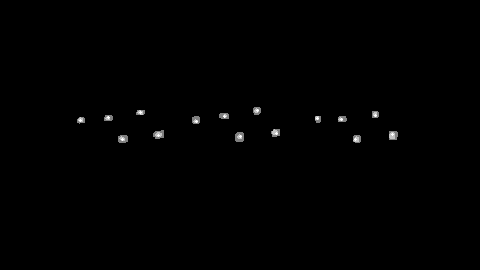
\includegraphics[scale=1.2]{results/t_in.png}
    \caption{Synthesized star image used as test input.}
    \label{res:t_in}
\end{figure}
\begin{figure}[h!]
    \centering
    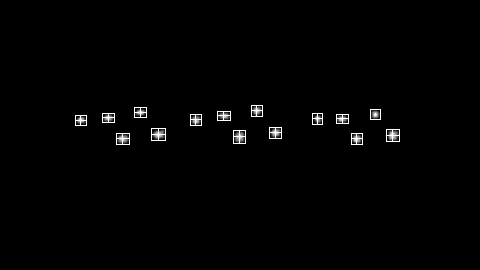
\includegraphics[scale=1.2]{results/t0.png}
    \caption{Run T1 output image.}
    \label{res:t0}
\end{figure}
\begin{figure}[h!]
    \centering
    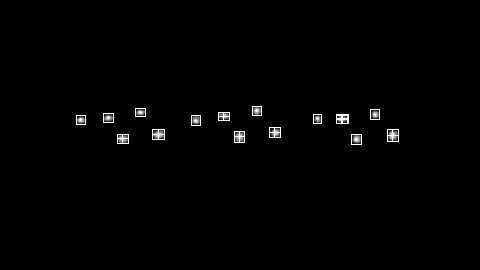
\includegraphics[scale=1.2]{results/t1.png}
    \caption{Run T2 output image.}
    \label{res:t1}
\end{figure}
The processing time for the test input runs are 0,1 ms apart, as seen in Table \ref{table:t_res}. The time difference originates from centroiding while other parts of the pre-processing pipeline remain unaffected by the foreground threshold increase. Since less pixels are processed in run T2, faster processing is expected. The increased number of weighted centroid calculations did also not contribute to any performance loss. The system is capable of a frame rate of 16,93 frames per second (FPS) in T1, and 16,96 FPS in T2. 

\subsection*{Sample 1}

Figure \ref{res:s0_in} shows the input image containing a moderate number of stars with mixed brightness levels. In contrast to the previously reviewed test input, this image consists of a realistic scenario of what an onboard image sensor captures. Also notable is that this is a good sample for star extraction and detection since there are numerous stars that are easily separated from the background and surrounding stars.
\par
The results show that all the extracted stars are within limits for weighted centroiding. After run S1.1 the feature threshold is decreased from 800 to 400 to extract more stars. This parameter change to increase star extraction is unsuccessful since Figure \ref{res:s0_2} shows the same number of extracted stars as Figure \ref{res:s0_1}.  
\par
A 0,12 ms difference in processing time between run S1.1 and S1.2, caused by the change in feature threshold, is observed in Table \ref{table:s0_res}. Compared to the test runs, shown in Table \ref{table:t_res}, no change can be seen in box filter processing time. The time difference in CCL is likely explained by the lower number of stars extracted, requiring less computation and rendering.
A frame rate of 17,12 FPS is achieved in S1.1, and 17,09 FPS in S1.2.

\begin{table}[h!]
    \centering
    \begin{tabular}{|p{0.8cm}|p{2.5cm}|p{2cm}||p{1.25cm}|p{1.25cm}|p{1.9cm}|p{1cm}|}
        \hline
        \textbf{Run ID}&\textbf{Foreground threshold$^{1}$}&\textbf{Feature threshold$^{1}$}&\textbf{CCL$^{2}$}&\textbf{Box filter$^{2}$}&\textbf{Centroid$^{2}$}&\textbf{Tot.$^{2}$}\\
        \hline
        \hline
        S1.1&50&800&39,38&18,84&0,19&58,41\\
        \hline
        S1.2&50&400&39,38&18,84&0,31&58,53\\
        \hline
    \end{tabular}
    \caption{$^{1}$Input parameter to the pre-processing pipeline, specified as pixel value. $^{2}$Performance metric of the pre-processing pipeline, measured in milliseconds. Data shows increase in centroid time when decreasing feature threshold.}
    \label{table:s0_res}
\end{table}
\begin{figure}[h!]
    \centering
    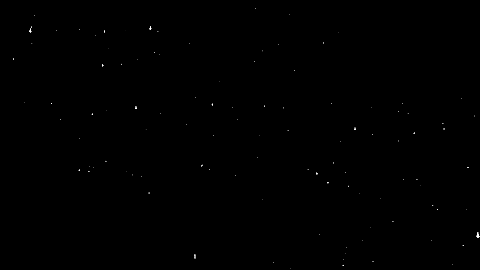
\includegraphics[scale=0.7]{results/s0_in.png}
    \caption{Sample 1 input image.}
    \label{res:s0_in}
\end{figure}
\begin{figure}[h!]
    \centering
    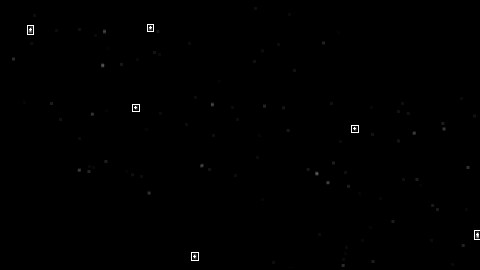
\includegraphics[scale=1.2]{results/s0_1.png}
    \caption{Run S1.1 output image.}
    \label{res:s0_1}
\end{figure}
\begin{figure}[h!]
    \centering
    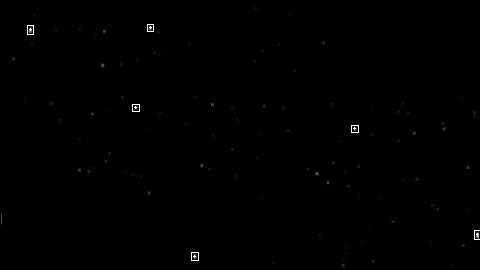
\includegraphics[scale=1.2]{results/s0_2.png}
    \caption{Run S1.2 output image.}
    \label{res:s0_2}
\end{figure}

\newpage
\subsection*{Sample 2}
Sample 2 input image has a few stars that are expected to be extracted, standing out with their brightness and dimensions. An anomaly, caused by the camera system or an optical artifact, is seen on the left side of the image, shown in Figure \ref{res:s1_in}. The pre-processing pipeline extracts the entire feature, including the anomaly, as seen in Figure \ref{res:s1_1} and \ref{res:s1_2}. In a star tracker this extraction is not valid since it gives a false representation of the celestial body in question.
\par
Run S2.1, shown in Figure \ref{res:s1_1}, contains four extracted stars using a foreground threshold of 40 and feature threshold of 800. This would otherwise be sufficient for star detection but since one of the stars is an anomaly the result is not reliable. The frame rate of S2.1 is 17,14 FPS.
\par
Run S2.2, shown in Figure \ref{res:s1_2}, contains in addition to the four in S2.1, three additional stars. With a decrease of foreground threshold of 25\%, from 40 to 30, the number of extracted stars increased by 75\%. The frame rate of S2.2 is 17,11 FPS.
\par
In the case of run S2.2 the 0,8 ms longer processing time, shown in Table \ref{table:s1_res}, compared to S2.1 is necessary to increase the quality of star extraction to an acceptable level.

\begin{table}[h!]
    \centering
    \begin{tabular}{|p{0.8cm}|p{2.5cm}|p{2cm}||p{1.25cm}|p{1.25cm}|p{1.9cm}|p{1cm}|}
        \hline
        \textbf{Run ID}&\textbf{Foreground threshold$^{1}$}&\textbf{Feature threshold$^{1}$}&\textbf{CCL$^{2}$}&\textbf{Box filter$^{2}$}&\textbf{Centroid$^{2}$}&\textbf{Tot.$^{2}$}\\
        \hline
        \hline
        S2.1&40&800&39,39&18,84&0,12&58,35\\
        \hline
        S2.2&30&800&39,39&18,84&0,2&58,43\\
        \hline
    \end{tabular}
    \caption{$^{1}$Input parameter to the pre-processing pipeline, specified as pixel value. $^{2}$Performance metric of the pre-processing pipeline, measured in milliseconds. Data shows that decreasing foreground threshold increases the processing time.}
    \label{table:s1_res}
\end{table}
\begin{figure}[h!]
    \centering
    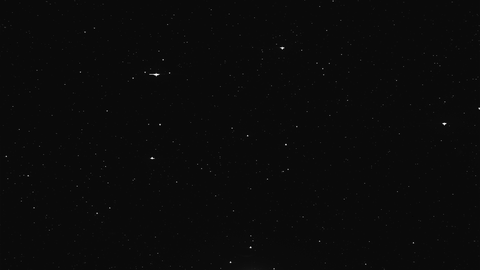
\includegraphics[scale=1.2]{results/s1_in.png}
    \caption{Sample 2 input image.}
    \label{res:s1_in}
\end{figure}
\begin{figure}[h!]
    \centering
    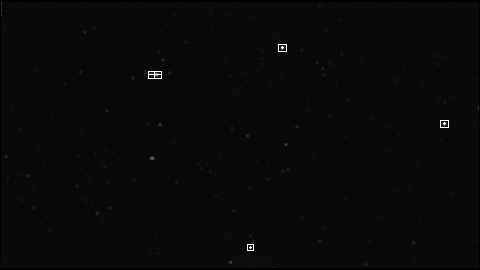
\includegraphics[scale=1.2]{results/s1_1.png}
    \caption{Run S2.1 output image.}
    \label{res:s1_1}
\end{figure}
\begin{figure}[h!]
    \centering
    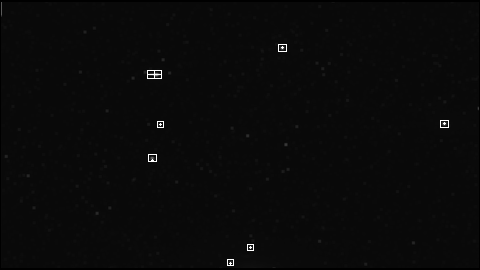
\includegraphics[scale=1.2]{results/s1_2.png}
    \caption{Run S2.2 output image.}
    \label{res:s1_2}
\end{figure}

\subsection*{Sample 3}
The Sample 3 input image, shown in Figure \ref{res:s2_in}, contains a cloud of faint and small stars. By tuning the input parameters correctly, this proves not to be any obstacle for star extraction as the S3.1 output image shows in Figure \ref{res:s2_1}.
\par
To extract the best selection of stars as detection candidates, the parameters can be tuned further. Since the dimensions of the extracted stars are relatively small, an increase in the foreground threshold is ruled out due to the effect seen in previous results, for example test input run T1. The feature threshold is thus increased to extract the brightest stars, keeping the dimensions and centroid precision. The result of this parameter tuning for S3.2 is shown in Figure \ref{res:s2_2}. The increase in the feature threshold in run S3.2 decreases the processing time by 0.2 ms, as shown in Table \ref{table:s2_res}. The frame rate of S3.1 is 17,09 FPS, and 17,14 FPS in S3.2.
\par
A notable aspect of the results is that the rendering of the centroid of a few stars is not visible. This is likely due to the small dimensions of the features, or a rounding error of the weighted centroid calculation.

\begin{table}[h!]
    \centering
    \begin{tabular}{|p{0.8cm}|p{2.5cm}|p{2cm}||p{1.25cm}|p{1.25cm}|p{1.9cm}|p{1cm}|}
        \hline
        \textbf{Run ID}&\textbf{Foreground threshold$^{1}$}&\textbf{Feature threshold$^{1}$}&\textbf{CCL$^{2}$}&\textbf{Box filter$^{2}$}&\textbf{Centroid$^{2}$}&\textbf{Tot.$^{2}$}\\
        \hline
        \hline
        S3.1&15&50&39,39&18,84&0,3&58,53\\
        \hline
        S3.2&15&100&39,39&18,84&0,1&58,33\\
        \hline
    \end{tabular}
    \caption{$^{1}$Input parameter to the pre-processing pipeline, specified as pixel value. $^{2}$Performance metric of the pre-processing pipeline, measured in milliseconds. Data shows that increasing feature threshold decreases processing time.}
    \label{table:s2_res}
\end{table}
\begin{figure}[h!]
    \centering
    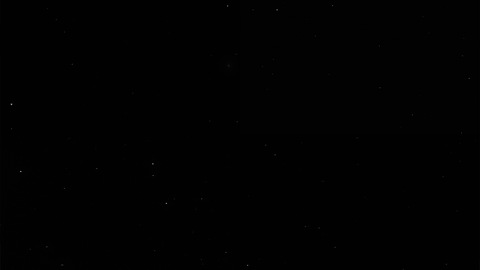
\includegraphics[scale=1.2]{results/s2_in.png}
    \caption{Sample 3 input image.}
    \label{res:s2_in}
\end{figure}
\begin{figure}[h!]
    \centering
    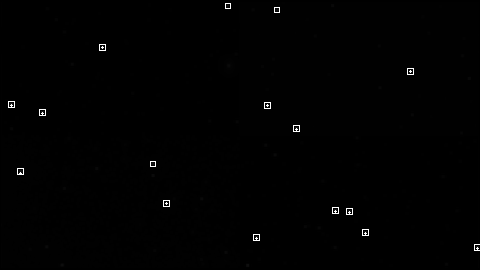
\includegraphics[scale=1.2]{results/s2_1.png}
    \caption{Run S3.1 output image.}
    \label{res:s2_1}
\end{figure}
\begin{figure}[h!]
    \centering
    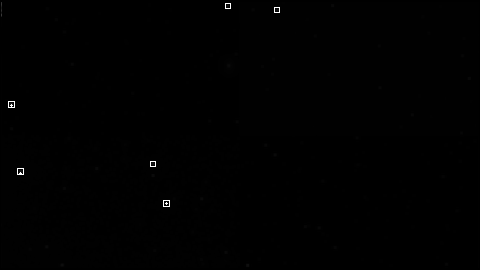
\includegraphics[scale=1.2]{results/s2_2.png}
    \caption{Run S3.2 output image.}
    \label{res:s2_2}
\end{figure}
\newpage
\subsection{Conclusion}
To summarize the results, the star tracker pre-processing pipeline works as intended, extracting stars from the input images. The procedure of the image processing system is clearly seen, when comparing input images to the output. 
\par
The box filter, for example, is visualized in the output of the test run seen in Figure \ref{res:t0}. The feature edges fade into the background more smoothly when compared to the input image, shown in Figure \ref{res:t_in}. The sample images, such as sample 3 shown in Figure \ref{res:s2_in}, benefit more clearly from this step of the pre-processing pipeline by expanding faint and small stars captured by the camera system as they are noticeably larger, and clearly extracted in the output, as seen in Figure \ref{res:s2_1}.
\par
The more complex CCL procedure is visualized by the frame around the stars, which is enabled by the algorithm successfully identifying the connected pixels. As the most critical part of the pre-processing pipeline, the lack of issues within the procedure is a priority. In addition to confirming the CCL results visually, the output metrics also indicate reliable results, with a consistent performance.
\par  
Weighted centroiding is also proven to work according to specification, shown by the results, such as Figure \ref{res:t1}. The dimension limitation of the stars enabling weighted centroiding is a drawback of the procedure. All input images, however, contain stars with dimensions fitting to the limits, making the procedure acceptable for star detection.
\par
The effect of the input parameter tuning is observable by the output images and metrics. An increase in the foreground threshold decreases the number of pixels included in a feature. This helped with features gaining a weighted centroid. This effect is shown in Figures \ref{res:t0} and \ref{res:t1}.
\par
A decrease in the foreground threshold is observed to increase the number of extracted stars, as shown in Figures \ref{res:s1_1} and \ref{res:s1_2}.
\par
The feature threshold shows a similar effect without any change in the number of pixels in each extracted feature. This effect is shown in Figures \ref{res:s2_1} and \ref{res:s2_2}.
\par
Based on these results, improvements could be made towards anomaly detection and centroid rendering. The results reinforce the justification for autonomous parameter tuning, by observing that small adjustments lead to significant changes, as seen in Table \ref{table:s1_res} and Figures \ref{res:s1_1} and \ref{res:s1_2}.
\par
Regardless of minor drawbacks and improvement points, the pre-processing pipeline is proven by the results to perform the intended task with a stable performance.

% anomaly detection vs star detection
% suitability for star detection, eg S2.2 not too many, not too few

% feature threshold increase -> ?
% feature threshold decrease -> ?
% foreground threshold increase -> ?
% foreground threshold decrease -> ?

% What is a result
% Insert input/ output images & metrics from client
\section{Pre-processing pipeline performance}
The performance of the pre-processing pipeline can be measured in the same way as any algorithm. The implemented performance measurement metric is execution time. Compared to a software based approach, it can be expected that the variation in execution time is smaller in a hardware based approach since there is no abstraction such as an operating system between the task and the computation element. Otherwise, a software based approach executed on an up-to-date CPU with multi-gigahertz clock speed is expected to perform a task in less time than an FPGA with a clock speed counted in megahertz. A software based equivalent of this FPGA-based approach would be an aerospace-grade embedded processor. An embedded processor would also be less performant than modern PC CPUs, in terms of execution time.
\par
The execution time comparison between the FPGA and a software based approach is executed on a 10th generation intel i5 CPU. 

\subsection{Software based approach}
To enable a comparison between the FPGA-design and a software based counterpart, a test bench in C++ was developed. The software test bench contains the same features, regarding image and parameter input and output metrics, as the FPGA-design \citep{cppImgProc}. Table \ref{table:res_sw} shows a summary of runs performed with the software based test bench using the same input images and parameters as used with the FPGA-based pre-processing pipeline. The results show noticeable differences in all output metrics. The complex hardware implementation of CCL is proven to be approximately 3 times slower than its software counterpart. On the other hand, the box filter is approximately 3 times faster when performed on the FPGA. The variation of difference in centroiding is larger since the test input runs T1 and T2 show an approximately 5 times faster centroiding performance by the software. The sample runs show a difference between 1 to 3 times faster performance by the software.
\par
The general conclusion when comparing the results of the software based approach in Table \ref{table:res_sw} to the results given by the FPGA is that the software is faster. When comparing the systems, the difference in CPU clock speed is significant. Thus another comparison can be made where the clock frequencies are normalized. Since most of the image processing related computation is performed using the 87 MHz clock on the FPGA, it is used for scaling the results. For each clock cycle on the FPGA, the Intel CPU performs approximately 23. Table \ref{table:res_sw_norm} shows the result using this ratio for normalizing the output metrics of the software based pre-processing pipeline. The performance of the Intel CPU with normalized clock speed shows CCL being approximately 7 times slower, while the box filter is over 60 times slower than the FPGA. Centroiding is calculated to be approximately 5 times slower. This proves the FPGA to be more efficient, regarding the number of operations on each clock cycle. It is notable that the two systems are not directly comparable despite normalizing the clock frequency due to differences in the arithmetics of the processing elements and the implementation of the pre-processing pipeline.

\begin{table}[h!]
    \centering
    \begin{tabular}{|p{0.8cm}|p{2.5cm}|p{2cm}||p{1.25cm}|p{1.25cm}|p{1.9cm}|p{1cm}|}
        \hline
        \textbf{Run ID}&\textbf{Foreground threshold$^{1}$}&\textbf{Feature threshold$^{1}$}&\textbf{CCL$^{2}$}&\textbf{Box filter$^{2}$}&\textbf{Centroid$^{3}$}\\
        \hline
        T1&50&300&12,1&55,3&149,1\\
        \hline
        T2&100&300&12,6&55,4&129,6\\
        \hline
        S1.1&50&800&12,6&53,4&76,1\\
        \hline
        S1.2&50&400&13,2&52,4&71,8\\
        \hline
        S2.1&40&800&12,5&55,7&78,7\\
        \hline
        S2.2&30&800&11,7&55,2&69,2\\
        \hline
        S3.1&15&50&12,2&53,6&83,1\\
        \hline
        S3.2&15&100&12,5&53,5&73,6\\
        \hline
    \end{tabular}
    \caption{$^{1}$Input parameter to the pre-processing pipeline, specified as pixel value. $^{2}$Performance metric of the pre-processing pipeline, measured in milliseconds. $^{3}$Performance metric of the pre-processing pipeline, measured in microseconds. \newline Results of the software based approach, produced by averaging the outputs of 10 runs. An Intel i5 CPU, running at 2GHz is used as the underlying hardware and Clang 11 as the compiler.}
    \label{table:res_sw}
\end{table}

\begin{table}[h!]
    \centering
    \begin{tabular}{|p{0.8cm}|p{2.5cm}|p{2cm}||p{1.25cm}|p{1.25cm}|p{1.9cm}|p{1cm}|}
        \hline
        \textbf{Run ID}&\textbf{Foreground threshold$^{1}$}&\textbf{Feature threshold$^{1}$}&\textbf{CCL$^{2}$}&\textbf{Box filter$^{2}$}&\textbf{Centroid$^{2}$}\\
        \hline
        T1&50&300&278,3&1271,9&3,4\\
        \hline
        T2&100&300&289,8&1274,2&3\\
        \hline
        S1.1&50&800&289,8&1228,2&1,8\\
        \hline
        S1.2&50&400&303,6&1205,2&1,7\\
        \hline
        S2.1&40&800&287,5&1281,1&1,8\\
        \hline
        S2.2&30&800&269,1&1269,6&1,6\\
        \hline
        S3.1&15&50&280,6&1232,8&1,9\\
        \hline
        S3.2&15&100&287,5&1230,5&1,7\\
        \hline
    \end{tabular}
    \caption{$^{1}$Input parameter to the pre-processing pipeline, specified as pixel value. $^{2}$Performance metric of the pre-processing pipeline, measured in milliseconds. \newline Results of the software based approach, produced by averaging the outputs of 10 runs and normalizing the clock speed.}
    \label{table:res_sw_norm}
\end{table}

% \subsection{CCL algorithm comparison}
% The CCL algorithm has many implementations, mostly within computer vision applications. There are thus many references that can be used for comparison.
% The implementa
% The most complex part of the image processing in the pre-processing pipeline is the CCL algorithm, making it a g

% Explain results
% What can results be compared to  
% Compare with CCL

% \begin{figure}[h]
%     \centering
%     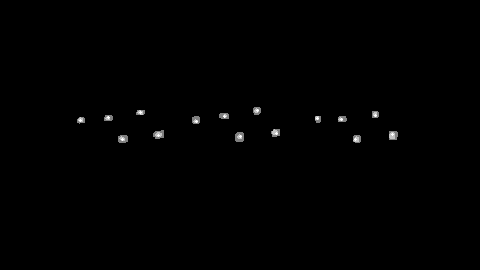
\includegraphics[scale=1.2]{results/t_in.png}
%     \caption{Synthesized star image used as test input.}
%     \label{res:t_in}
% \end{figure}
% \begin{figure}[h]
%     \centering
%     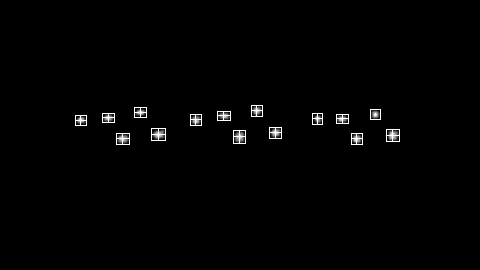
\includegraphics[scale=1.2]{results/t0.png}
%     \caption{Run T1 output image.}
%     \label{res:t0}
% \end{figure}
% \begin{figure}[h]
%     \centering
%     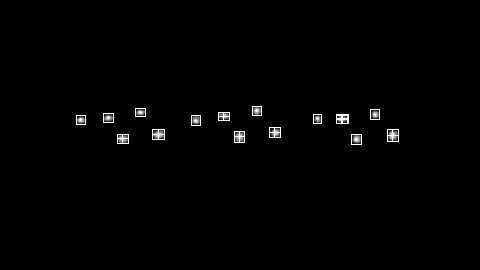
\includegraphics[scale=1.2]{results/t1.png}
%     \caption{Run T2 output image.}
%     \label{res:t1}
% \end{figure}
% \begin{figure}[h]
%     \centering
%     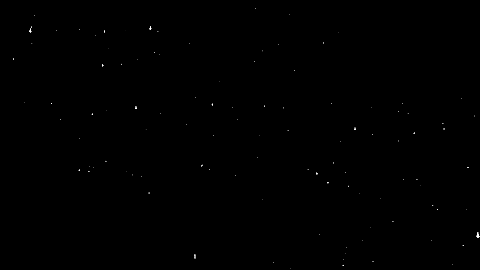
\includegraphics[scale=0.7]{results/s0_in.png}
%     \caption{Sample 1 input image.}
%     \label{res:s0_in}
% \end{figure}
% \begin{figure}[h]
%     \centering
%     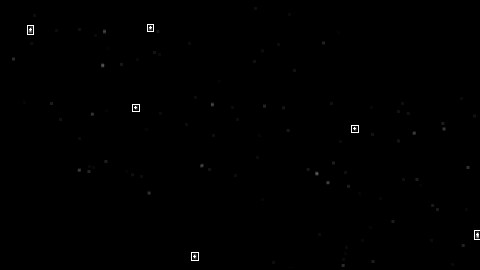
\includegraphics[scale=1.2]{results/s0_1.png}
%     \caption{Run S1.1 output image.}
%     \label{res:s0_1}
% \end{figure}
% \begin{figure}[h]
%     \centering
%     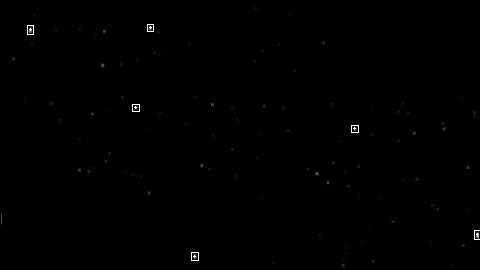
\includegraphics[scale=1.2]{results/s0_2.png}
%     \caption{Run S1.2 output image.}
%     \label{res:s0_2}
% \end{figure}
% \begin{figure}[h]
%     \centering
%     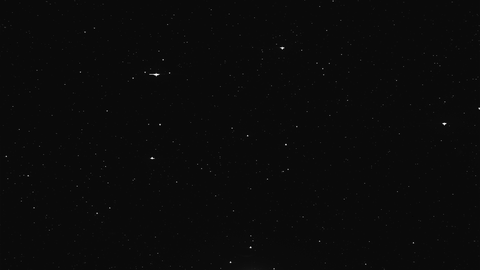
\includegraphics[scale=1.2]{results/s1_in.png}
%     \caption{Sample 2 input image.}
%     \label{res:s1_in}
% \end{figure}
% \begin{figure}[h]
%     \centering
%     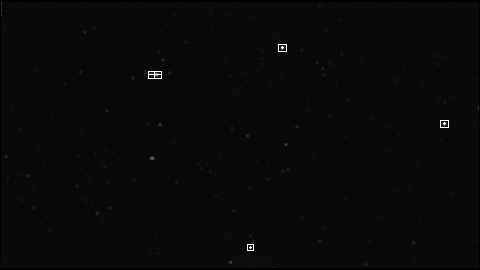
\includegraphics[scale=1.2]{results/s1_1.png}
%     \caption{Run S2.1 output image.}
%     \label{res:s1_1}
% \end{figure}
% \begin{figure}[h]
%     \centering
%     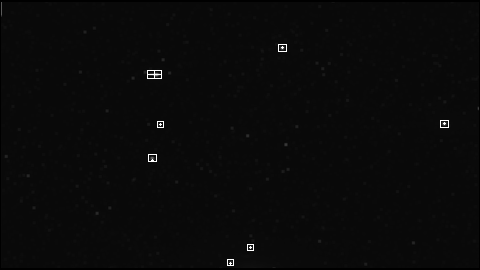
\includegraphics[scale=1.2]{results/s1_2.png}
%     \caption{Run S2.2 output image.}
%     \label{res:s1_2}
% \end{figure}
% \begin{figure}[h]
%     \centering
%     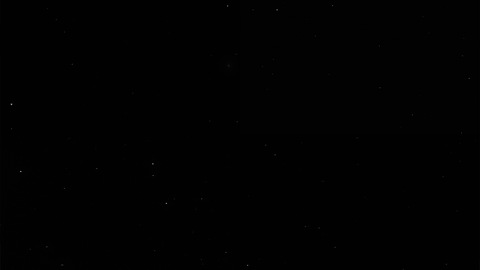
\includegraphics[scale=1.2]{results/s2_in.png}
%     \caption{Sample 3 input image.}
%     \label{res:s2_in}
% \end{figure}
% \begin{figure}[h]
%     \centering
%     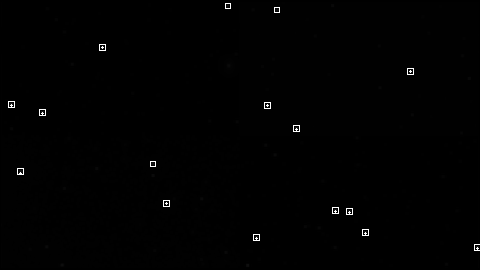
\includegraphics[scale=1.2]{results/s2_1.png}
%     \caption{Run S3.1 output image.}
%     \label{res:s2_1}
% \end{figure}
% \begin{figure}[h]
%     \centering
%     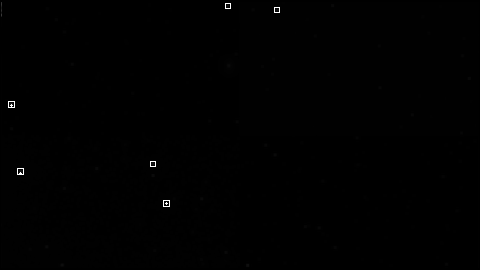
\includegraphics[scale=1.2]{results/s2_2.png}
%     \caption{Run S3.2 output image.}
%     \label{res:s2_2}
% \end{figure}

\chapter{Review and reflection}

In this thesis a star tracker pre-processing pipeline has been developed with a technology used on the forefront of image processing and computer vision in general. As the pre-processing pipeline is essentially a sequence of image processing algorithms, the implementation on an FPGA platform is an option worth consideration when designing a star tracker system. This thesis gives an overview of the required components and technologies to develop such a system. Beyond implementing the star tracker pre-processing pipeline in a star tracker system, this study gives a complete reference from digital circuitry to system level design, to help with comparing other platform options. 
\par

\section{System requirements}
The gap between a functioning algorithm and its implementation in an FPGA design regarding technology is vast. The challenge in implementing a pre-processing pipeline to an FPGA design is divided between solving problems within the development of the image processing algorithm and computer hardware design practices. This resulted in some compromises and recommendations with respect to the system requirements in Table \ref*{table:sysreq}.
\par
The implementation of requirement \hyperref[req3.2]{3.2}, centroiding of stars, could be revised to increase the flexibility regarding feature size. The development was focused on the computation of the weighted centroid, leaving the operational functionality as a lower priority.
\par
Requirement \hyperref[req3.3]{3.3}, involving error handling, could be implemented more thoroughly in the FPGA design. Even though error handling is enabled by exposing parameters in the pre-processing pipeline, some error correction could also be implemented.
\par

\section{FPGA design}
The FPGA design is reviewed based on reports generated by Vivado. Timing and power constraints are commonly placed on FPGA designs to meet certain requirements. The focus in this thesis is to implement the pre-processing pipeline, giving less attention on meeting constraints. Optimizations to meet power consumption and timing requirements can be developed based on the current state of the design.
\par
The reports generated by Vivado for this review focus on the resource utilization shown in Table \ref*{table:fpga_res} and Figure \ref*{fig:fpga_util}.

\begin{table}[h]
    \centering
    \begin{tabular}{|c|c|c|c|c|}
        \hline
        \textbf{LUT}& \textbf{SLICEM}& \textbf{SLICEL}& \textbf{DSP blocks}& \textbf{BRAM Arrays}\\
        \hline
        24131&2046&4690&5&142\\
        \hline
    \end{tabular}
    \caption{FPGA resource utilization. The number of LUTs, slices, DSP blocks and BRAM arrays are listed.}
    \label{table:fpga_res}
\end{table}

\begin{figure}[h]
    \centering
    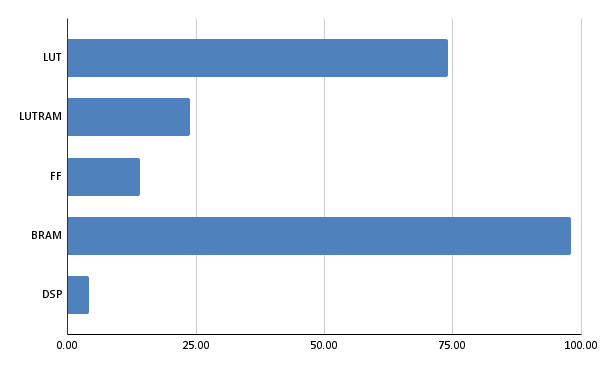
\includegraphics[scale=0.65]{figures/utilization.png}
    \caption{Utilization \% of available FPGA resources. Total LUT utilization and LUTs used as storage mechanism, LUTRAM, are shown. Together with flip flop utilization, the internal utilization of CLBs is described. The more specialized resources, BRAM and DSPs, are also reported.}
    \label{fig:fpga_util}
\end{figure}

As seen in Table \ref*{table:fpga_res}, the size of the FPGA design is reported to be 24131 LUTs, and 9242 flip flops, contributing to the 83 \% slice utilization on the FPGA. The ratio between flip flops and LUTs is large due to the nature of the CLBs in Xilinx 7 series FPGAs, where each CLB contains more flip flops than LUTs.
\par
In addition to LUTs, Figure \ref*{fig:fpga_util} shows that also BRAM utilization is high, at almost 100 \%. A part of the BRAM is utilized by the FIFO buffer used for image transfer, while the remaining parts are used by the line buffers. The FIFO buffer uses 38 Kb BRAM arrays and the line buffer uses 18 Kb arrays. The line buffer uses the 18 Kb arrays to enable the multiport feature of the storage mechanism.
\par
The high utilization means that the FPGA part used for this design is at the limit, making it a good fit for the current state of the design. It also means that adding features would be difficult without additional resources. An integration of the pre-processing pipeline thus requires a larger FPGA with more resources.
\par
The low level storage mechanisms have a low utilization compared with the BRAM and overall LUT utilization. This can be seen in Table \ref*{table:fpga_res}, where the count of SLICEM-type slices is relatively low compared to SLICEL. This correlates highly with the LUTRAM utilization in Figure \ref*{fig:fpga_util}.
\par
The low utilization of DSP blocks is not unexpected because the parts of the design that most likely use these blocks are not parallelized. The pre-processing pipeline performance could be increased with higher utilization of the DSP blocks, the penalty being a higher power consumption. 
\par
The conclusion of the FPGA design, based on the reports generated by Vivado, is that the high degree of utilization of resources prohibits adding features requiring a large amount of LUTs or BRAM on the same FPGA. Optimizing the design to use more DSP blocks could release more LUTs to use.
\par
The estimated power consumption can be seen in Figure \ref*{fig:fpga_power}, showing a total power consumption of 1,053 watt (W). This reinforces the confidence of using an FPGA as computing platform for the star tracker pre-processing pipeline, as a low power consumption is preferred. For comparison, the 2 GHz Intel i5 CPU used for the software based pre-processing pipeline in the previous chapter consumes 28 W. Although this means that the Intel CPU has a smaller power consumption per clock cycle, the total power consumption is considerably lower.
\begin{figure}[h]
    \centering
    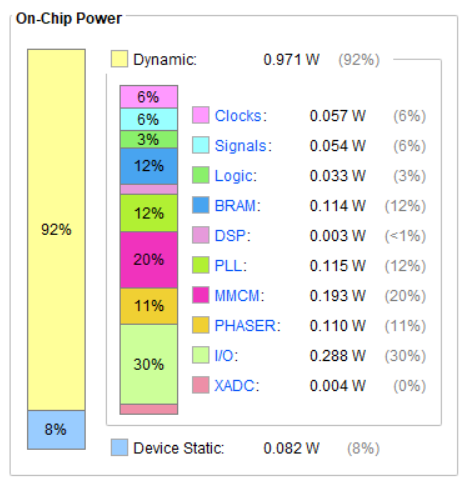
\includegraphics[scale=0.9]{figures/power_report.PNG}
    \caption{Summary of power consumption showing estimated usage by each section of the FPGA. A total power consumption of 1,053 W is consumed when the pre-processing pipeline is operational and 0,082 W in idle mode.}
    \label{fig:fpga_power}
\end{figure}

% Streamlined CCL, preparing for centroid & feature detection

\chapter{Summary in Swedish - Svensk sammanfattning}
\section*{Implementering av FPGA-baserad förbearbetningssekvens för stjärnspårare}

Algoritmer som kräver bästa möjliga prestanda använder sig ofta av en hårdvarubaserad lösning istället för en tillämpning i mjukvara. Inom flyg- och rymdindustrin är det ofta den mest optimerade lösningen som är det enda alternativet. I denna avhandling utvecklas en hårdvarubaserad implementering av en förbearbetningsmodul för ett stjärnspårarsystem tillsammans med Aboa Space Research Oy. Som grund för arbetet fungerar StreakDet-mjukvaran som behandlar bilder från omloppsbanan för analys. 
\par
Ett stjärnspårarsystem används vanligen på rymdfarkoster som ett navigations\-medel. Stjärnspårarens uppgift är att förse diverse system i rymdfarkosten med positionsdata. För att implementera detta vanligen mjukvarubaserade system i hårdvara krävs det, utöver bildbehandlingsalgoritmerna från StreakDet, en mängd stödande arkitektur så som kommunikations- och minnessystem.
\par
Specialiserad processeringshårdvara är, till skillnad från allmännyttiga processor\-enheter som t.ex. en CPU, avsedd för att lösa problem inom en viss domän. En GPU är ett exempel på specialiserad processeringshårdvara, vars uppgift är att lösa problem inom datorgrafik, som ofta innebär matrisberäkningar. För att tillfredsställa behovet av skräddarsydd och omprogrammerbar hårdvara kan en FPGA användas. I och med att en FPGA kan programmeras för att utföra matrisberäkningar har teknologin tillsammans med GPUn blivit vanlig inom accelerering av AI och kryptografi.
\par
En FPGA består huvudsakligen av logikblock, det vill säga CLB, och ett så kallat interconnect, som används för att koppla ihop logikblocken. Figur \ref{fig:2} visar ett antal CLB sammankopplade i ett nätverk och FPGAns kanter bestående av portar för externa signaler. En FPGA-design beskriver hur logikblocken ska konfigureras och kopplas ihop. Detta är jämförbart med ett schema som beskriver hur en integrerad krets ser ut och fungerar. Ett CLB består av varierande element beroende hurdan uppgift de har. Vissa CLB är ämnade för lagring av data, medan andra är ämnade för att utföra logiska operationer. \citep{XilVivado}
\par
Det huvudsakliga verktyget för att skapa en FPGA-design är ett HDL. Verilog och VHDL är exempel på ett sådant. Till skillnad från programmeringsspråk beskriver man med hjälp av HDL hur en digital krets fungerar från ett dataflödesperspektiv. En kretsbeskrivning i ett HDL programmeras på en FPGA genom ett antal processer, som tar i beaktande den ifrågavarande FPGAns egenskaper. Denna process kan även användas för att tillåta simulering av designen, då är processen i regel avsevärt mycket kortare.
\par
Genom användning av IP-block kan hårdvarumoduler distribueras och återanvändas. Vanligen implementeras moduler så som minneskontroller och kommunikationsmoduler som IP-block i en FPGA-design. IP-block har i allmänhet en varierande grad av transparens gällande dess interna design. Det möjliggör distribution av designen, som ofta sker via patentlicenser. \citep{XilVivado} \citep{EERefBook}
\par
Systemspecifikationen för förbearbetningssekvensen beskriver hur det FPGA-baserade systemet fungerar som helhet. Specifikationen är konstruerad på basis av StreakDet och diskussioner med Aboa Space Research Oy, och redogörs för i Tabell \ref{table:sysreq}.
\par
Det centrala i systemet är FPGAn vars uppgift är att utvinna stjärnor från bilder. Bilden förväntas härstamma från rymdfarkostens bildsensor, som är riktad mot en känd riktning. Denna implementering sker från ett integrerat perspektiv, där bildens ursprung inte har en inverkan. Specifikationen delar in helheten i en klient och en FPGA-modul, där klientens uppgift är att förse FPGA-modulen med bild och konfiguration. Den ifrågavarande FPGA-modulen är bestämd att vara av modell Opal Kelly XEM7305, som har en Xilinx 7-Series FPGA, en klockkrets, USB C-gränssnitt med kontroller, samt SDRAM. Resultatskraven för bildanalysen lägger vikt på vidare processering av den utvunna informationen, så som lagring av koordinaterna och centroiden av stjärnorna inom bildramen. Andra väsentliga funktioner som krävs är möjlighet för validering och verifiering av systemet. Både klienten och FPGA-modulen har en bidragande roll i detta.
\par
FGPA-modulen Opal Kelly XEM7305 med sitt subsystem presenteras för att ge bakgrund för den implementerade designen. Figur \ref{fig:xemOverview} visar ett blockdiagram över denna modul. Systemspecifikationen anger en kommunikationskanal för delat minne och en konfiguration av förbearbetningssekvensen, vilket USB C-gränssnittet uppfyller. Gränssnittet är kopplat till Cypress FX3-kontrollern, som implementerar protokollen för kommunikationssystemet. FPGA-designen når kontrollern genom ett IP-block. \citep{XEM7305Man}
\par
Tre olika minnessystem används för lagring av data på FPGA-modulen. Det största minnet består av en SDRAM-modul med 4Gb kapacitet. Minnet nås genom ett kontrollergränssnitt, som är implementerat i ett IP-block. Det näst största minnet är BRAM, vars storlek beror på den valda konfigurationen. Det förekommer i 36Kb minnesblock som kan kombineras eller spjälkas beroende på behovet. Denna minnesresurs finns inom själva FPGAn, men skilt från logikblocken. Distribuerat RAM är den minsta minnesresursen och även den snabbaste. Det är inbakat i logikblocken, vilket innebär en avvägning mellan resursanvändningen inom FPGAn. \citep{XEM7305Man}
\par
Systemet hålls synkroniserat med hjälp klocksignalen från en 200 MHz oscillatorkrets. Utöver själva FPGAn använder sig också SDRAM-minnet av samma klocksignal. Minneskontrollern fördelar klocksignalen till en 87 MHz signal som driver minnet och synkroniserar operationerna. Cypress FX3 USB C-kontrollern använder sig av en skild oscillatorkrets, som genererar en 100,8 MHz signal. \citep{XEM7305Man}
\par
Stjärnspårare och astronomisk navigering möjliggörs av uppfinningar inom tillämpad vetenskap, med betoning på astrofysik. Olika processeringsenheter har ofta en avgörande uppgift inom dess moderna tillämpningar. Ett objekts position i rymden kan beskrivas på olika sätt. Det valda sättet beror på objektet och omloppsbanan. Positionen för objekt i låg bana runt jorden beskrivs ofta med hjälp av det ekvatoriella koordinatsystemet. Deklination och rektascension används för att uttrycka positionen, vilket kan jämföras med longitud och latitud på jorden. \citep{SatDesgin}
\par
Attityden för ett objekt i rymden beskriver dess lutning i jämförelse med en referensram. En attitydmatris är ett sätt att uttrycka objektets attityd och består av $3\times3$ flyttal som representerar vinklarna mot varje plan. Figur \ref{fig:orbit} visar ett diagram med en satellit, dess koordinater, attitydmatris och bildsensorns synfält. \citep{StRef}
\par
En stjärnspårare är ett instrument vars uppgift är att bidra med positionsdata, som koordinater och attityd genom att utvinna och känna igen stjärnor från en bild. Systemet består i regel av en kamera och en dator. Kameran tar bild av stjärnorna, överför datan till datorn som utvinner stjärnorna och jämför dem mot en stjärnkatalog. Stjärnkatalogen innehåller position för kända stjärnor, vilket används för beräkning av position och attityd. \citep{SatDesgin}
\par
Den implementerade förbearbetningssekvensen är dokumenterad utgående från kraven i systemspecifikationen och hur de satisfierats. Helheten illustreras i Figur \ref{fig:overview}, som visar de väsentliga komponenterna hos klienten och FPGAn. Det centrala i projektet är att genomföra bildanalysen för att bidra med data för igenkänning av stjärnor. Därför är systemet utvecklat med syfte att integreras i en större helhet, vilket oundvikligt medför kompromisser som t.ex. påverkar användbarheten.
\par
Hårdvarudesignen är utvecklad i Verilog, med hjälp av Xilinx Vivado-utvecklings\-miljön. Vivado bygger designen tillsammans med IP-blocken och konfigurationsfilerna för Opal Kelly XEM7305-FPGAn, som producerar en bitstream fil. Denna fil används sedan för att programmera FPGAn. Programmeringen genomförs av klienten, eftersom FPGAn måste alltid omprogrammeras då den kopplas till ström.
\par
Händelseförloppet från användarens synvinkel för systemet är kortfattat följande: Ström och datalänk kopplas till FPGA-modulen. Klienten öppnar förbindelsen till modulen och programmerar FPGA-designen. Bilden överförs till FPGA-modulens SDRAM. Parametrarna för förbearbetningssekvensen programmeras och processen kan köras igång. Resultat i form av bild och logg kan sedan läsas från FPGAn.
\par
En översikt av FPGA-designen visas i Figur \ref{fig:fpga_design}, där FPGAns interna och externa block är kartlagda. Det programmerbara gränssnittet som används för styrning och kommunikation med FPGAn kallas okHost. Den innehåller logik och gränssnitt för Cypress FX3 USB C-kontrollern och oscillatorkretsen. Från okHost kopplas databussar till IP-block med kommunikations- och dataöverföringssyften. IP-blocket Opal Kelly register bridge tillåter en gemensam synkroniserad $32 \times 32$-bit registerbank mellan FPGAn och klienten. Registerbanken används främst för lagring av parametrar och resultatdata. Wire In- och Wire Out-blocken innehåller ett 32-bit register var, som används för asynkron kommunikation mellan klienten och FPGAn. Dessa block används som kommunikationskanal för styrning av systemet. Överföringen av bilddata hanteras av Pipe In- och Pipe Out-blocken. Dessa block kopplas ihop med buffertar och SDRAM-minnet för att överkomma skillnader i klockfrekvens och busstorlek. Bilddatan använder två ytterligare buffertmekanismer som möjliggör behandlingsalgoritmernas funktion. En linjebuffert lagrar tre kolumner av bilden, medan kernelbufferten lagrar en $3 \times 3$ matris med bilddata. Figur \ref{fig:mem_overview} beskriver lagringssystemet för bilden inom förbearbetnings\-sekvensen. \citep{stpp}
\par
Förbearbetningssekvensen går enligt följande: Bilden filtreras med ett så kallat boxfilter, vars uppgift är att förbereda för CCL-processen. Figur \ref{fig:box_filter} visar resultatet då boxfiltret tillämpats på en del av bilden. Eftersom CCL kräver en binär bild, dvs. varje pixel representeras av antingen 0 eller 1, tillämpar man en tröskel på varje pixel. Denna tröskel är parametriserad och styrs från klienten. Sedan tillämpas CCL-processen på bilden som sammankopplar närliggande pixlar till objekt. Objektens mått och ljusstyrka lagras under processen. Sedan beräknas centroiden för objekten. En viktad centroid beräknas för objekt vars geometri är inom vissa mått. Övriga objekt beräknas en oviktad centroid. Centroidberäkningen efterföljs av renderingen av resultaten med de utvunna objekten och desras centroider, till SDRAM-minnet. Klienten kan sedan läsa bilden från SDRAM minnet. Figur \ref{fig:centroids} visar exempel på utvunna stjärnor och centroider. \citep{stpp}
\par
Klienten består av en Java-applikation med ett grafiskt användargränssnitt. 
Genom det kan användaren konfigurera och styra förbearbetningssekvensen. Enkla verktyg för jämförelse och analys är implementerade, vilket bidrar till att uppfylla specifikationskraven. \citep{stpp}
\par
Resultat av förbearbetningssekvensen presenteras genom exempelanvändning av systemet. Figur \ref{res:t_in} visar testdata som är genererade på basis av bilder från StreakDet. Figur \ref{res:t0} visar resultatet från förbearbetningssekvensen där det framkommer att alla stjärnor har plockats ur den inmatade bilden.  Figur \ref{res:t1} visar resultatet från samma inmatade bild, med en annan parameterkonfiguration. Konfigurationerna och resultatdata redogörs för i Tabell \ref{table:t_res}.
\par
Analys av resultatdatan och bilderna leder till slutsatsen att förbearbetningssekvensen beter sig som förväntat och väldigt förutsägbart i frågan om temporal prestation. När systemet jämförs med en mjukvaruvariant är den FPGA-baserade varianten snabbare då klockfrekvenserna normaliseras.
\par
För att undersöka och reflektera över systemet ytterligare kan Vivado användas för att ge en uppfattning angående FPGA-designen. Det framkommer att mängden programmerbara resurser på FPGAn utnyttjas till en hög grad, vilket lämnar relativt lite överloppsutrymme i kretsen. En estimering av FPGAns strömförbrukning ges av Vivado, som påstår den totala förbrukningen vara 1.053 W. En jämförelse med processorn som användes för att exekvera mjukvaruvarianten visar att FPGAn har betydligt lägre strömförbrukning. Med tanke på strömförbrukning per klockcykel har den mjukvaruexekverande processorn bättre prestanda.


\addcontentsline{toc}{chapter}{Bibliography}

\bibliographystyle{unsrt}
\bibliography{references}

\end{document}